\documentclass[11pt]{article}

%% Journal of Forecasting, free-format submission (Wiley author guidelines).
%% Build: pdflatex -> bibtex -> pdflatex -> pdflatex

\usepackage[a4paper,margin=2.5cm]{geometry}
\usepackage[T1]{fontenc}
\usepackage{lmodern}
\usepackage{setspace}
\usepackage{lineno}
\usepackage{booktabs}
\usepackage{threeparttable}
\usepackage{array}
\usepackage{amsmath}
\usepackage{graphicx}
\usepackage[authoryear,round]{natbib}
\usepackage{xurl}
\usepackage[hidelinks]{hyperref}
\usepackage{orcidlink}
\setlength{\emergencystretch}{2em}

\newcommand{\pkg}[1]{\textsf{#1}}
\newcommand{\proglang}[1]{\textsf{#1}}
\newcommand{\code}[1]{\texttt{#1}}
\providecommand{\sectionref}[1]{Section~\ref{#1}}
\providecommand{\tableref}[1]{Table~\ref{#1}}
\providecommand{\figureref}[1]{Figure~\ref{#1}}
\providecommand{\appendixref}[1]{Appendix~\ref{#1}}

\begin{document}

%% ------------------------------------------------------------------ title page
\begin{titlepage}
\begin{center}
{\LARGE\bfseries Foundation or Formula? A Simulation-Based Comparison of Google's TimesFM-3 and
Classical Time-Series Models\par}
\vspace{1.5em}
{\large Ebrahim Khaled Ebrahim\,\orcidlink{0009-0006-7839-8778}$^{1}$,
Somaia Mohamed Ali\,\orcidlink{0009-0002-0940-8451}$^{2}$ and
Ahmed El-Kotory\,\orcidlink{0009-0000-1485-0768}$^{3}$\par}
\vspace{1em}
{\small $^{1}$Department of Applied Statistics, Faculty of Business, Alexandria University,
Alexandria, Egypt\\
$^{2}$Department of Statistics, Alexandria University, Alexandria, Egypt\\
$^{3}$Alexandria University, Alexandria, Egypt\par}
\end{center}

\vspace{1.5em}
\noindent\textbf{Correspondence:} Ebrahim Khaled Ebrahim, Department of Applied Statistics,
Faculty of Business, Alexandria University, Alexandria, Egypt.
Email: \href{mailto:ebrahimkhaled@alexu.edu.eg}{ebrahimkhaled@alexu.edu.eg}

\medskip
\noindent\textbf{Running title:} TimesFM-3 versus classical models

\medskip
\noindent\textbf{Keywords:} time-series foundation models; zero-shot forecasting; simulation
study; forecast evaluation; intermittent demand; exponential smoothing

\medskip
\noindent\textbf{Data availability statement:} The complete research compendium is archived on Zenodo at \code{10.5281/zenodo.22681072} (concept DOI, resolving to all versions): the pre-registered protocol, the deviation log, the entire pipeline, the per-series metrics for all 129\,600 evaluations, the raw forecasts and quantiles, every figure and the manuscript source. All data in the simulation tier are generated by that code from documented seeds; the real-data tier uses the publicly available M4 competition data \citep{makridakis2020m4}, which the code re-fetches, with the seeded 1\,000-series sample included so the analysis reproduces exactly.

\medskip
\noindent\textbf{Funding statement:} No funding was received for this work.

\medskip
\noindent\textbf{Conflict of interest disclosure:} The authors declare no conflicts of interest.

\medskip
\noindent\textbf{Ethics approval statement:} Not applicable; the study uses simulated data and
the publicly available M4 competition data, and involves no human participants.

\medskip
\noindent\textbf{Permission to reproduce material from other sources:} Not applicable.
\end{titlepage}

\onehalfspacing
\linenumbers

\begin{center}
{\Large\bfseries Foundation or Formula? A Simulation-Based Comparison of Google's TimesFM-3 and
Classical Time-Series Models\par}
\end{center}

\begin{abstract}
Time-series foundation models such as Google's TimesFM-3, a 330-million-parameter model released
in August 2026, forecast series they were never trained on. Whether such models should replace
classical methods such as ARIMA and exponential smoothing is difficult to settle on public
benchmarks, because only about 6\% of the datasets used to evaluate published models are absent
from every model's pre-training corpus. The aim of this exploratory study is to describe, under
controlled conditions, how TimesFM-3 behaves relative to classical forecasting methods and in
which regimes it may be preferred. The evaluation data
are generated from nine known processes, so the foundation model cannot have seen the series and
the classical models are correctly specified by construction. Across 7\,200 series, four lengths
and a pre-registered protocol, neither family dominates. TimesFM-3 has the lowest mean absolute
scaled error (MASE) in 16 of 36 design cells and wins 113 of 132 significant pairwise comparisons;
only automatic ARIMA performs comparably. TimesFM-3 is never more than 1.31 times worse than the
best method in a cell, whereas every classical method is at least 2.2 times worse in some cell.
With four seasonal cycles observed, automatic ARIMA is 21--24\% more accurate. On intermittent
demand, TimesFM-3 outperforms six Croston-family methods under MASE but not under the root mean
squared scaled error. A robustness study in which every series draws its own parameters, and the
data have heavy tails, outliers or a seasonal period that must be estimated, preserves these
conclusions, with TimesFM-3 at most 1.51 times worse than the best method. In a feature space,
this randomised design covers 81\% of M4 monthly series, and results on 1\,000 of them agree.
TimesFM-3 is 103 times faster per series than automatic ARIMA, but its weights are licensed for
non-commercial use only. Because TimesFM-3 is a black box whose pre-training data cannot be
inspected, the study characterises its behaviour, not the reasons for it, and its conclusions are
conditional on the regimes examined.
\end{abstract}

\section{Introduction}
\label{sec:intro}

Time-series foundation models are large neural networks that are pre-trained on many series
and then applied to new series without task-specific training. On 31 August 2026 Google Research
released TimesFM-3, the third generation of its TimesFM family \citep{timesfm3blog}: a
330-million-parameter decoder-only transformer, the first member of the family designed for
\emph{multivariate} forecasting, which its developers report as the top-ranked pre-trained model
on three public benchmarks for both point and probabilistic accuracy. \sectionref{sec:timesfm}
describes the model in detail.

For applied forecasting, the relevant question is not whether such a model ranks first on a
leaderboard but whether it should be used, in preference to a classical method such as ARIMA, for
the series at hand. The two families also differ in more than accuracy: in computational cost, in
the interpretability of their parameters, in the theoretical basis of their prediction intervals
and, as \sectionref{sec:licence} discusses, in the terms under which they may be used.

Published benchmark evidence is poorly suited to answering this question. \citet{meyer2025leakage} traced the data lineage of 22 time-series
foundation models and found that of the 401 datasets used to evaluate them, only about 6\%
had never appeared in \emph{any} model's pre-training or fine-tuning corpus. They further
showed that even a 0.1\% overlap between pre-training and test data can move mean absolute
percentage error by 8 to 29 percentage points, and that leakage need not be direct: a model
trained on temporally overlapping, causally related series inherits an advantage on a target
series it has never seen. A benchmark result obtained on a public dataset is therefore a
measurement of unknown provenance. In addition, foundation-model evaluations have been
criticised for comparing against de-ensembled or under-tuned classical baselines rather
than the combinations that win forecasting competitions \citep{makridakis2020m4}.

This study addresses both objections by generating its own evaluation data. Under a known
data-generating process (DGP), two conditions hold that cannot hold on a public benchmark.
First, the foundation model cannot have seen the series, because the series did not exist before
the experiment was run. Second, the classical model can be made \emph{correctly specified by
construction}: when the data are generated by an ARIMA(1,1,1) process with drift, the model
family searched by AutoARIMA contains the true process, and only its parameters remain to be
estimated.

One distinction is essential to the interpretation of the results.
What the design excludes is contamination at the level of the \emph{realisation}: these specific
series did not exist before the experiment ran, so no pre-training corpus can contain them, and
the leakage documented by \citet{meyer2025leakage} is impossible by construction. What the design
does \emph{not} exclude is familiarity at the level of the \emph{family}. TimesFM-3 is trained on
more than a trillion time points drawn from real-world \emph{and synthetic} corpora
\citep{timesfm3blog}, and synthetic pre-training data for time-series models is commonly
generated from exactly the parametric processes D1--D7 use. The model may therefore arrive
already fluent in ARMA-like and seasonal structure without ever having seen these draws.

This is a boundary of what the design can establish. Whether family-level familiarity affects
the results cannot be tested here, because the pre-training corpus is not available for
inspection. If it does, it would be expected to help TimesFM-3 most on D1--D5, the processes where
a classical model is correctly specified and where the classical methods win; under that
conjecture the gap measured there would understate rather than overstate the accuracy TimesFM-3
gives up. The conjecture is stated for transparency and no conclusion relies on it.

The design therefore replaces the general question of which method is better with two specific
questions:

\begin{itemize}
\item how much accuracy does zero-shot TimesFM-3 give up on the classical model's
      \emph{home ground}, where the parametric form is exactly right; and
\item how much does it gain where no classical form is right---structural breaks,
      nonlinear saturation, intermittent demand, changing volatility?
\end{itemize}

Both questions are addressed across nine DGPs, four series lengths from 24 to 200
observations, three forecast horizons and 7\,200 simulated series, by comparing TimesFM-3 with seasonal naive, Theta,
AutoETS, AutoARIMA and an equal-weight combination of the last three. The protocol, including
the hypotheses, was pre-registered before any forecast was produced, and every departure from
it is recorded.

The aim of the study is therefore exploratory: to describe, under controlled experimental
conditions, how the accuracy of TimesFM-3 relative to classical methods varies across regimes, and
to derive from that description diagnostic baselines for when it may be preferred and when it
should not. It proposes no new estimator, test or theory.

The design can establish what TimesFM-3 does; it cannot establish why. The behaviour of a classical
model can be traced to its equations and estimated parameters, whereas TimesFM-3 is a black box:
its 330 million parameters have no individual interpretation, and its pre-training corpus is not
available for inspection. Explanations of its behaviour offered in this paper, for example that
its forecasts behave as if they drew on a prior over common series shapes, are therefore
interpretations consistent with the measurements, not findings. The measurements themselves are
also bounded. They concern one model, one checkpoint, univariate zero-shot use and the regimes
examined, and they do not support general statements about foundation models as a class. Within
these bounds the controlled design offers what public benchmarks cannot: a known ground truth,
series the model cannot have seen, and a pre-registered analysis.

The remainder of the paper is organised as follows. \sectionref{sec:timesfm} describes
TimesFM-3. \sectionref{sec:design} sets out the design of the simulation study, and
\sectionref{sec:results} reports its results. \sectionref{sec:robustness} examines how
representative the simulated series are of real data and whether the conclusions survive randomly
drawn parameters, heavy-tailed noise, outliers and an estimated seasonal period.
\sectionref{sec:realdata} applies the comparison to
monthly series from the M4 competition. \sectionref{sec:operational} examines computational cost,
licensing, interpretability and the basis of prediction intervals. \sectionref{sec:discussion}
assesses the pre-registered hypotheses and presents practical recommendations and limitations,
and \sectionref{sec:conclusion} concludes. Computational details are given in
\sectionref{sec:repro}, and results under the mean absolute percentage error in
\appendixref{app:mape}.

\subsection{Related work}
\label{sec:related}

The foundation-model literature for time series is young and moving quickly. TimesFM
\citep{das2024timesfm}, Chronos \citep{ansari2024chronos} and Moirai \citep{woo2024moirai}
established that a single pre-trained network can forecast unseen series without task-specific
training, and GIFT-Eval \citep{aksu2024gifteval} supplied a common benchmark. The critical
literature has grown alongside it: \citet{meyer2025leakage} on contamination, and
\citet{adler2026calibrated} on calibration, who evaluated five foundation models against two
baselines on six univariate datasets and found that calibration error grows with forecast
length.

The present study complements that of \citet{adler2026calibrated} in three respects. Their
evidence comes from public datasets and therefore inherits the contamination problem, whereas the
data here are generated. They summarise reliability with calibration \emph{metrics}, whereas this
study combines interval coverage with pre-registered \emph{hypothesis tests} on accuracy
differences, with control of multiplicity. Finally, their study predates TimesFM-3, the first
natively multivariate member of the family.

Applied comparisons of foundation models with classical methods on real data are appearing in
several fields; \citet{chu2026influenza}, for example, compare six foundation models, TimesFM
among them, with SARIMA and regression models on eleven years of influenza surveillance data.
Such studies answer whether a model works on one data set; they cannot say why, because the
generating mechanism is unknown. The design of the present study follows an established pattern
in this journal, in which a controlled simulation over several data-generating processes is
followed by an empirical application: \citet{berger2025deep} compares recurrent neural networks
with ARMA models on simulated and observed return series, \citet{chu2026intervals} assess
machine-learning and classical prediction intervals under nonlinear, seasonal and heteroskedastic
processes, and \citet{lisi2025multiple} evaluate seasonal ARIMA extensions against TBATS and
related methods by simulation before two applications. The question of whether simulated series
resemble real ones is addressed, as in \citet{kang2017instance} and \citet{talagala2023metalearning},
by placing both in a common space of time-series features (\sectionref{sec:representativeness}).

The classical side of the comparison is deliberately strong. AutoARIMA and AutoETS follow the
Hyndman--Khandakar automatic selection procedures \citep{hyndman2008forecast,
hyndman2002statespace}, Theta is the method that won M3 \citep{assimakopoulos2000theta}, and
the equal-weight combination is included because combinations, not individual models, are the
standard against which competition entries are judged \citep{makridakis2020m4}. Evaluation
follows the scale-free conventions of \citet{hyndman2006mase} and the M5 competition
\citep{makridakis2022m5, makridakis2022m5unc}, and the design avoids the
evaluation pitfalls catalogued by \citet{hewamalage2023evaluation}.

\section{The TimesFM-3 model}
\label{sec:timesfm}

This section summarises the properties of TimesFM-3 that bear on the comparison: its
architecture (\sectionref{sec:tfm-architecture}), its pre-training data
(\sectionref{sec:tfm-data}), and the released checkpoint together with the configuration used in
this study (\sectionref{sec:tfm-config}).

\subsection{Architecture}
\label{sec:tfm-architecture}

TimesFM-3 is the third generation of the TimesFM family of decoder-only time-series foundation
models developed at Google Research \citep{das2024timesfm, timesfm3blog}. Each input series is
normalised and divided into non-overlapping patches of 32 time points, and each patch is
embedded as a token. The released model stacks 20 transformer layers with model dimension 1280
and 16 attention heads, for a total of about 330 million parameters
\citep{timesfm3blog, timesfm3card}.

The principal change from earlier generations is native support for multivariate forecasting.
Layers of causal attention along the time axis alternate with layers of full attention across
variates, so that several target series, past covariates and past--future covariates can be
processed jointly \citep{timesfm3blog}. Forecasts are produced non-autoregressively: a contiguous
patch masking scheme allows the whole horizon to be generated in a single forward pass
\citep{timesfm3blog}, and the released configuration emits output patches of 64 time points
\citep{timesfm3card}. For each step of the horizon the model outputs nine quantiles, from the
10th to the 90th percentile, and its point forecast is the median of these quantiles
\citep{timesfm3blog, timesfm3repo}.

\subsection{Pre-training data}
\label{sec:tfm-data}

TimesFM-3 was pre-trained on a corpus of more than one trillion time points that combines
real-world and synthetic series \citep{timesfm3blog}. According to the model card, the
real-world component includes the GIFT-Eval pre-training corpus \citep{aksu2024gifteval},
Wikipedia page views up to November 2023 and Google Trends queries up to the end of 2022, and it
is supplemented by synthetic and augmented series \citep{timesfm3card}. Two consequences matter
for this study. Public benchmarks may be contained in the corpus, which is why the primary
evaluation uses generated data (\sectionref{sec:dgps}). And because part of the corpus is
synthetic, the model may already be familiar with the parametric families used here even though
it cannot have seen the particular realisations, as discussed in \sectionref{sec:intro}.

\subsection{Released checkpoint and configuration used in this study}
\label{sec:tfm-config}

The pre-trained weights are distributed through the Hugging Face Hub under the repository
identifier \code{google/\allowbreak timesfm-3.0-pytorch} and are loaded with version 3.0.1 of the
\pkg{timesfm} \proglang{Python} package \citep{timesfm3repo, timesfm3card}. They are released
under a non-commercial licence, whose implications are discussed in \sectionref{sec:licence}. In
this study the model is used zero-shot: it receives only the raw context of each series, with no
fine-tuning, no covariates and no information about the seasonal period, and it returns the
median point forecast and the nine deciles for each step of the horizon. Because no quantile
outside the 10th and 90th percentiles is available, the widest prediction interval that can be
formed from its output is the nominal 80\% interval (\sectionref{sec:evaluation}).

TimesFM-3 is a black box in the sense that matters for interpretation, though not in the sense
that matters for reproducibility. Its weights, architecture and inference code are public, so every
forecast in this study can be reproduced exactly by any reader, and the checkpoint is fixed, so the
results do not depend on a service that may change. What is not available is the pre-training
corpus itself and any interpretation of the 330 million parameters comparable to the coefficients
of an ARIMA model. The study therefore treats TimesFM-3 as a
forecasting procedure whose properties are to be \emph{measured}, in the same way that a
forecaster evaluates any method whose internal workings cannot be inspected: by its accuracy
and calibration on data whose generating mechanism is known. This is the purpose of the
controlled design in \sectionref{sec:design} and of the robustness study in
\sectionref{sec:robustness}. Such measurements describe the model's behaviour; they do not
reveal the mechanism that produces it.

\section{Design of the simulation study}
\label{sec:design}

This section describes the data-generating processes (\sectionref{sec:dgps}), the forecasting
methods compared (\sectionref{sec:methods}), and the evaluation measures and inferential
procedures (\sectionref{sec:evaluation}).

\subsection{Data-generating processes}
\label{sec:dgps}

Nine processes were chosen to span the range from ``a classical model is exactly right'' to
``no classical model is right''. \tableref{tab:dgps} lists them. Each series is generated at
length $n + H$ with $H = 12$; the first $n$ observations form the context supplied to every
method, and the final 12 are held out as the truth. One realisation of each process is shown
in \figureref{fig:series}.

\begin{table}[!htbp]
\centering
\begin{threeparttable}
\caption{The nine data-generating processes and their parameters.}
\label{tab:dgps}
\small\setlength{\tabcolsep}{4pt}
\begin{tabular}{llll}
\toprule
ID & Data-generating process & Parameters & Correctly specified by \\
\midrule
D1 & AR(1)                        & $\phi = 0.7$                                & ARIMA \\
D2 & ARMA(1,1)                    & $\phi = 0.6$, $\theta = 0.4$                & ARIMA \\
D3 & ARIMA(1,1,1) with drift      & $\phi = 0.5$, $\theta = 0.3$, drift $0.3$   & ARIMA \\
D4 & SARIMA(1,0,0)(1,1,0)$_{12}$  & $\phi = 0.6$, $\Phi = 0.5$                  & ARIMA \\
D5 & ETS(A,A,A)                   & $\alpha = 0.3$, $\beta = 0.01$, $\gamma = 0.2$ & ETS \\
D6 & Local level with a break     & break at $0.7n$, jump $10\sigma$            & neither \\
D7 & Logistic growth              & $K = 180$, $r = 0.08$, floor $20$           & neither \\
D8 & Intermittent demand          & $P = 0.3$, size $1 + \mathrm{Pois}(4)$      & neither \\
D9 & AR(1) with GARCH(1,1) errors & $\phi = 0.6$, $a = 0.1$, $b = 0.85$         & ARIMA in mean \\
\bottomrule
\end{tabular}
\begin{tablenotes}[flushleft]\footnotesize
\item \textit{Note:} The last column states which classical family is correctly specified by
construction; for D6--D8 none is, and for D9 the conditional mean is correctly specified while
the conditional variance is not. In D6, $\sigma$ is the standard deviation of the observation
noise.
\end{tablenotes}
\end{threeparttable}
\end{table}

\begin{figure}[!htbp]
\centering
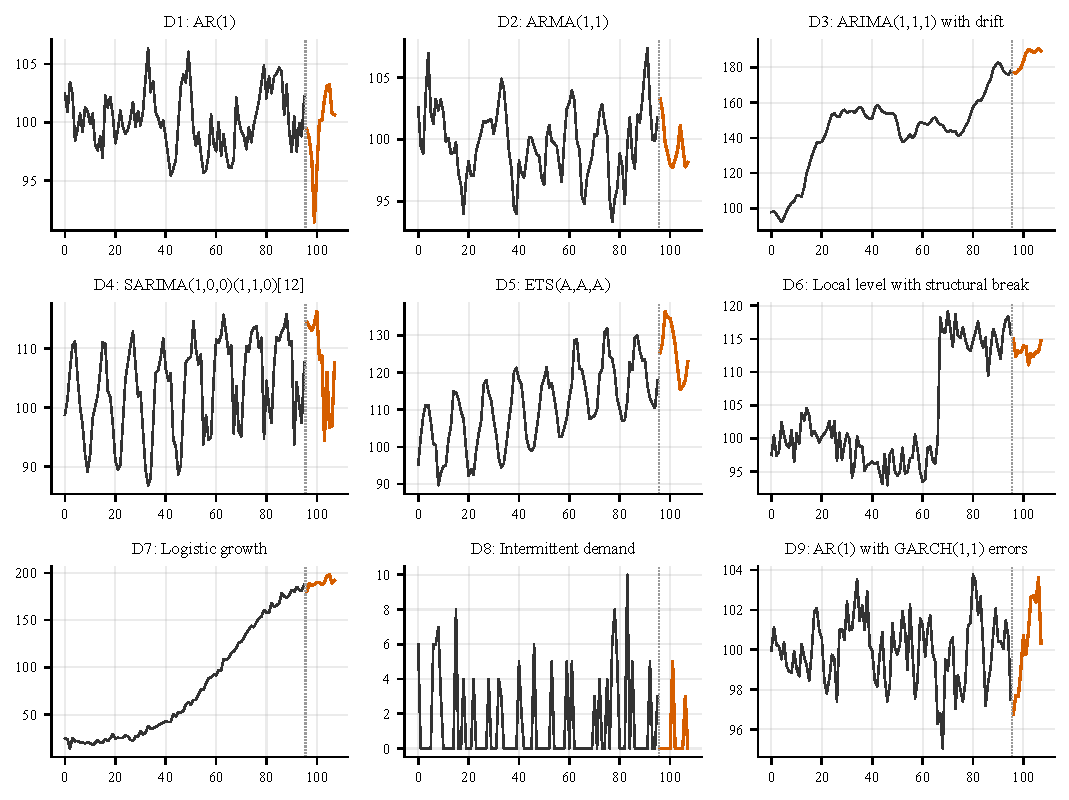
\includegraphics[width=\textwidth]{../figures/fig1_example_series.pdf}
\caption{One realisation of each data-generating process at $n = 96$. The context supplied to
every method is in grey and the held-out horizon in colour, separated by the dotted line.}
\label{fig:series}
\end{figure}

The parameter values in \tableref{tab:dgps} were fixed in the pre-registered protocol before any
forecast was produced. They were not taken from a single earlier study; each was chosen so that
its process represents its regime unambiguously, according to four criteria. First, the linear
processes D1--D4 and the conditional mean of D9 use moderate coefficients, none larger than 0.7
in absolute value, so that their autoregressive and moving-average polynomials lie well inside
the stationarity and invertibility regions \citep{brockwell2016introduction} and no automatic
method is assessed at parameter values close to the boundaries of those regions. Second, the
smoothing parameters of the ETS process D5 lie inside the usual region $0 < \beta < \alpha < 1$,
$0 < \gamma < 1 - \alpha$ \citep{hyndman2008ets}, with a small trend parameter so that the level
remains positive over the longest series. Third, the three processes outside the classical
families are placed firmly within the regimes they represent. The break in D6 equals ten standard
deviations of the observation noise, so that its occurrence is not in doubt and the comparison
concerns adaptation to the break rather than its detection \citep{pesaran2007breaks}. D7 follows
the logistic curve, the standard model of saturating growth in diffusion forecasting
\citep{meade2006diffusion}. In D8 a demand occurs with probability 0.3, so the mean interval
between demands is $1/0.3 \approx 3.3$ periods, and demand sizes $1 + \mathrm{Pois}(4)$ have a
squared coefficient of variation of $4/25 = 0.16$; against the cut-offs of 1.32 and 0.49
proposed by \citet{syntetos2005categorization}, the process is intermittent rather than lumpy,
which is the regime for which Croston's method and its variants were developed
\citep{croston1972}. The GARCH(1,1) errors of D9 \citep{bollerslev1986garch} have $\omega = 0.1$
and persistence $a + b = 0.95$, a strongly persistent but covariance-stationary conditional
variance \citep{engle1986persistence}, and GARCH(1,1) is a standard benchmark specification in
volatility forecasting \citep{hansen2005garch}. Fourth, every series has a level of about 100,
or a positive lower asymptote in D7, so that percentage error measures are defined except where
zeros are intrinsic to the process (D8). Two values, the trend parameter of D5 and the lower
asymptote of D7, were adjusted for this reason before any forecast was produced, and both changes
are recorded in the deviation log. Because the conclusions could depend on these particular
values, \sectionref{sec:robustness} repeats the comparison with parameters drawn at random from
wide ranges.

Three further design choices require explanation.

The structural break in D6 is placed inside the \emph{context}, at $0.7n$, not inside the
forecast window. A break in the held-out window is unforecastable by any method, so a design
that placed it there would measure only which method is the most conservative. Placing it in
the context instead poses a question every method can answer: having seen the level shift, do
you forecast from the new level or revert towards the old one?

The inflection of the logistic curve in D7 sits at $0.6(n+H)$, so the held-out window falls in
the saturating arm. Any method that fits a linear drift should overshoot here; this is the
behaviour the process is designed to reveal.

Series lengths are $n \in \{24, 48, 96, 200\}$. The shortest length is deliberately demanding: at
$n=24$ with a seasonal period of 12, a seasonal model has only two complete cycles from which
to estimate its seasonal structure. As \sectionref{sec:results} shows, this separates two
things that are usually conflated---whether a model is correctly \emph{specified}, and whether
it is \emph{estimable} from the data available.

Two hundred replications are generated per (DGP, length) cell, giving
$9 \times 4 \times 200 = 7\,200$ series. Each series is seeded deterministically from its own
identifiers, so it is reproducible independently of core count or execution order.

\subsection{Forecasting methods}
\label{sec:methods}

No method receives manual tuning: each classical model uses its own automatic order and
parameter selection, which is the comparison a practitioner would face. TimesFM-3 is used
zero-shot, as described in \sectionref{sec:tfm-config}, and the classical models are fitted with
\pkg{StatsForecast} \citep{statsforecast}.

The equal-weight combination of Theta, AutoETS and AutoARIMA is included deliberately.
Foundation-model evaluations are frequently criticised for comparing against individual classical
methods, whereas the classical state of the art is a combination \citep{makridakis2020m4, petropoulos2022theory};
omitting it would bias the design in favour of the foundation model. Standard implementations of these
classical benchmarks follow established principles \citep{hyndman2021fpp}.

The construction of the combination's \emph{predictive distribution} is stated explicitly,
because one recommendation depends on it. Its point forecast is the equal-weight mean of the three members, but
its quantiles are obtained by averaging the members' quantile functions decile by decile
(vincentization) rather than by mixing their distributions. The two differ: vincentization
produces a narrower predictive distribution than a mixture when the members disagree about
location, so the combination's intervals here are sharper---and, as \sectionref{sec:realdata}
shows, better calibrated on M4---than a mixture would have given. Any comparison of the
combination's intervals against TimesFM-3's is a comparison against this particular construction.

One asymmetry in the design favours the classical methods.
Every classical method is given the \emph{true} seasonal period as an input---$m = 12$ on D4 and
D5, $m = 1$ elsewhere---whereas TimesFM-3 receives only the raw context, with no frequency label
and no indication that the series is seasonal at all. The classical methods thus begin with a
piece of oracle knowledge the foundation model must infer. This reflects ordinary practice, since
an analyst usually does know whether data are monthly, and the same $m$ is used for the MASE
denominator so the metric is unaffected. But it means the seasonal results (D4, D5) are, if
anything, generous to the classical methods. \sectionref{sec:robustness} removes this advantage
by repeating the comparison with a period that the classical methods must estimate.

\subsection{Evaluation measures and statistical inference}
\label{sec:evaluation}

Point accuracy is measured primarily by the mean absolute scaled error
\citep[MASE;][]{hyndman2006mase}, with the root mean squared scaled error (RMSSE) and sMAPE
as secondary measures. All three are scaled by the in-sample seasonal-naive error computed on
the context, so they are comparable across processes of different magnitude.
Let $y_{T+1}, \dots, y_{T+H}$ denote the observed future values over forecast horizon $H$, and
$\hat{y}_{T+1}, \dots, \hat{y}_{T+H}$ the point forecasts generated from the observed context $y_1, \dots, y_T$
(where $T = n$). The Mean Absolute Scaled Error is defined as:
\begin{equation}
\label{eq:mase}
\text{MASE} = \frac{\frac{1}{H}\sum_{h=1}^H |y_{T+h} - \hat{y}_{T+h}|}{\frac{1}{T-m}\sum_{t=m+1}^T |y_t - y_{t-m}|},
\end{equation}
where $m$ is the seasonal period ($m = 12$ on D4 and D5; $m = 1$ elsewhere). The Root Mean Squared Scaled
Error is similarly:
\begin{equation}
\label{eq:rmsse}
\text{RMSSE} = \sqrt{\frac{\frac{1}{H}\sum_{h=1}^H (y_{T+h} - \hat{y}_{T+h})^2}{\frac{1}{T-m}\sum_{t=m+1}^T (y_t - y_{t-m})^2}},
\end{equation}
and the symmetric Mean Absolute Percentage Error is:
\begin{equation}
\label{eq:smape}
\text{sMAPE} = \frac{200\%}{H} \sum_{h=1}^H \frac{|y_{T+h} - \hat{y}_{T+h}|}{|y_{T+h}| + |\hat{y}_{T+h}|}.
\end{equation}

MAPE is reported only in \appendixref{app:mape}. It is undefined when an actual value is zero,
it is asymmetric between over- and under-forecasts, and on the intermittent process D8 it is
simply unusable---a point the results make concrete rather than assert
\citep{hyndman2006mase, kolassa2016count}.

Probabilistic accuracy is evaluated under strictly proper scoring rules \citep{gneiting2007scoring},
measured by the mean pinball loss over the nine deciles $\tau \in \{0.1, 0.2, \dots, 0.9\}$, scaled by
the same in-sample denominator:
\begin{equation}
\label{eq:spl}
\text{SPL} = \frac{\frac{1}{9H} \sum_{\tau} \sum_{h=1}^H \max\{\tau(y_{T+h} - \hat{q}^{(\tau)}_{T+h}),\, (1-\tau)(\hat{q}^{(\tau)}_{T+h} - y_{T+h})\}}{\frac{1}{T-m}\sum_{t=m+1}^T |y_t - y_{t-m}|},
\end{equation}
where $\hat{q}^{(\tau)}_{T+h}$ denotes the estimated $\tau$-quantile forecast. This is complemented by the
empirical coverage and mean width of the nominal 60\% and 80\% prediction intervals to evaluate
probabilistic calibration and sharpness \citep{gneiting2007calibration}.
The choice of 60\% and 80\%, rather
than the more familiar 90\% or 95\%, is forced by the comparison itself: TimesFM-3 emits only
the nine deciles, so a 90\% interval cannot be formed from its output. Comparing a classical
90\% interval against a foundation-model interval constructed by extrapolation would not be a
like-for-like comparison, so the widest interval both families can express, $[q_{0.1},
q_{0.9}]$, is used as the widest interval reported. Classical quantiles are obtained from
prediction intervals at levels 20, 40, 60 and 80, which map exactly onto the same deciles.

Differences in accuracy are tested formally. Within each (DGP, length, horizon)
cell, TimesFM-3 is compared with each classical method by a paired Wilcoxon signed-rank test
\citep{wilcoxon1945} on per-replication MASE differences, accompanied by the Hodges--Lehmann
estimate of the median difference \citep{hodges1963} and the median MASE ratio, so that a
difference which is statistically detectable but practically negligible is visible as such.
Multiplicity across cells is controlled by the Benjamini--Hochberg procedure at a false
discovery rate of 0.05 \citep{benjamini1995fdr}.

The Diebold--Mariano test \citep{diebold1995comparing}, the usual instrument in this
literature, is not used, for the following reasons. DM is built for an autocorrelated sequence of loss differentials
generated by a single series over time. In the simulation tier the replications within a cell
are independent draws from the DGP, so a paired rank test across replications is the
appropriate tool and DM would misstate the dependence structure. The pre-registered protocol
did reserve DM for the real-data tier, where rolling origins do generate such a sequence---but
the realised design yields only three origins per series, giving a per-series DM statistic two
degrees of freedom and no useful power, even under small-sample corrections \citep{harvey1997testing}. Applying it instead across the 1\,000 series would be
worse still, since those are indexed by series identifier rather than by time, and a
serial-correlation correction over an arbitrary ordering is not a test at all. DM is therefore
dropped in both tiers rather than reported with a caveat, and the departure is recorded.

\section{Simulation results}
\label{sec:results}

This section reports the results of the simulation study. \sectionref{sec:overall} summarises
overall accuracy and the pairwise comparisons, \sectionref{sec:effects} reports effect sizes and a
sensitivity analysis, and \sectionref{sec:estimability} examines the role of estimability.
\sectionref{sec:regimes} and \sectionref{sec:croston} analyse the seasonal and intermittent
regimes, the latter with purpose-built intermittent-demand baselines. \sectionref{sec:horizon}
and \sectionref{sec:coverage} consider accuracy across forecast horizons and the coverage of
prediction intervals, and \sectionref{sec:combination} and \sectionref{sec:mape} report two
robustness analyses. Throughout, statements about TimesFM-3 describe the behaviour of its
forecasts; where an explanation is offered, it is an interpretation, since the model's internal
workings cannot be inspected.

The design yields 7\,200 series and, with six methods and three horizon slices, 129\,600
per-series evaluations. \tableref{tab:mase} reports mean MASE over the full horizon
$h = 1,\dots,12$, and \figureref{fig:ratio} displays the accuracy of TimesFM-3 relative to the
best classical method in each cell on a logarithmic scale, which shows the pattern across
processes and lengths more directly than the table.

% generated by code/09_make_tables.py -- do not edit by hand
\begin{table}[!htbp]
\centering
\begin{threeparttable}
\caption{Mean MASE over $h = 1,\dots,12$ across 200 replications per cell.}
\label{tab:mase}
\small\setlength{\tabcolsep}{3pt}
\begin{tabular}{llrrrrrr}
\toprule
DGP & $n$ & Seas.\ naive & Theta & AutoETS & AutoARIMA & Combin. & \textbf{TimesFM-3} \\
\midrule
D1 (ARIMA) & 24 & 1.646 & 1.682 & 1.568 & 1.485 & 1.538 & \textbf{1.417} \\
 & 48 & 1.625 & 1.586 & 1.570 & 1.415 & 1.478 & \textbf{1.381} \\
 & 96 & 1.626 & 1.572 & 1.564 & 1.324 & 1.435 & \textbf{1.307} \\
 & 200 & 1.615 & 1.576 & 1.576 & 1.266 & 1.417 & \textbf{1.254} \\
\addlinespace
D2 (ARIMA) & 24 & 1.905 & 2.003 & 1.886 & 1.708 & 1.788 & \textbf{1.675} \\
 & 48 & 1.838 & 1.860 & 1.834 & 1.575 & 1.688 & \textbf{1.518} \\
 & 96 & 1.810 & 1.812 & 1.811 & 1.517 & 1.643 & \textbf{1.455} \\
 & 200 & 1.922 & 1.919 & 1.921 & \textbf{1.374} & 1.654 & 1.383 \\
\addlinespace
D3 (ARIMA) & 24 & \textbf{4.411} & 4.483 & 4.892 & 5.275 & 4.659 & 4.656 \\
 & 48 & 4.252 & \textbf{4.179} & 4.547 & 4.679 & 4.313 & 4.274 \\
 & 96 & 4.125 & 4.135 & 3.938 & 3.940 & \textbf{3.871} & 4.023 \\
 & 200 & 4.512 & 4.427 & 4.275 & \textbf{4.195} & 4.199 & 4.297 \\
\addlinespace
D4 (ARIMA) & 24 & \textbf{1.029} & 4.146 & 3.602 & 2.284 & 3.084 & 1.321 \\
 & 48 & 1.021 & 1.944 & 1.720 & \textbf{1.014} & 1.395 & 1.295 \\
 & 96 & 1.005 & 2.910 & 2.407 & \textbf{0.886} & 1.839 & 1.124 \\
 & 200 & 1.053 & 4.155 & 1.085 & \textbf{0.886} & 1.700 & 1.161 \\
\addlinespace
D5 (ETS) & 24 & \textbf{1.139} & 3.154 & 3.025 & 1.574 & 2.474 & 1.152 \\
 & 48 & 1.108 & 0.956 & 0.741 & \textbf{0.717} & 0.731 & 0.815 \\
 & 96 & 1.076 & 0.757 & 0.761 & 0.732 & \textbf{0.713} & 0.761 \\
 & 200 & 1.040 & 0.759 & 0.681 & \textbf{0.626} & 0.645 & 0.689 \\
\addlinespace
D6 (none) & 24 & 0.801 & 1.327 & \textbf{0.766} & 0.802 & 0.837 & 0.807 \\
 & 48 & 0.947 & 1.115 & 0.869 & 0.925 & 0.924 & \textbf{0.825} \\
 & 96 & 1.006 & 0.963 & 0.905 & 0.920 & 0.916 & \textbf{0.865} \\
 & 200 & 0.934 & 0.840 & \textbf{0.825} & 0.833 & 0.827 & 0.844 \\
\addlinespace
D7 (none) & 24 & 5.417 & 3.179 & 1.272 & \textbf{1.083} & 1.680 & 1.142 \\
 & 48 & 4.243 & 2.262 & 1.602 & 1.076 & 0.970 & \textbf{0.751} \\
 & 96 & 1.655 & \textbf{0.821} & 1.305 & 1.329 & 1.097 & 0.959 \\
 & 200 & \textbf{0.917} & 1.301 & 0.966 & 0.994 & 0.954 & 0.933 \\
\addlinespace
D8 (none) & 24 & 1.019 & 0.999 & 1.047 & 0.996 & 1.010 & \textbf{0.780} \\
 & 48 & 1.066 & 0.984 & 0.988 & 0.962 & 0.974 & \textbf{0.708} \\
 & 96 & 0.932 & 0.923 & 0.926 & 0.924 & 0.923 & \textbf{0.683} \\
 & 200 & 1.005 & 0.943 & 0.939 & 0.939 & 0.940 & \textbf{0.694} \\
\addlinespace
D9 (ARIMA (mean only)) & 24 & 1.547 & 1.518 & 1.454 & 1.372 & 1.404 & \textbf{1.321} \\
 & 48 & 1.588 & 1.486 & 1.476 & 1.244 & 1.353 & \textbf{1.239} \\
 & 96 & 1.430 & 1.342 & 1.333 & \textbf{1.098} & 1.213 & 1.104 \\
 & 200 & 1.577 & 1.503 & 1.504 & \textbf{1.190} & 1.341 & 1.200 \\
\bottomrule
\end{tabular}
\begin{tablenotes}[flushleft]\footnotesize
\item \textit{Note:} Lower is better; the best method in each row is in bold. The family in parentheses after each process label is the one correctly specified for it by construction.
\end{tablenotes}
\end{threeparttable}
\end{table}


\begin{figure}[!htbp]
\centering
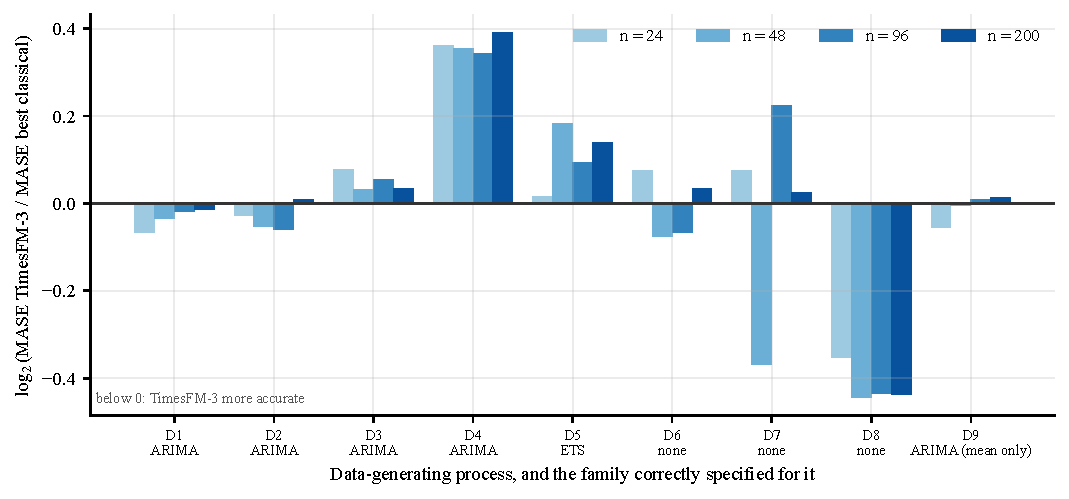
\includegraphics[width=\textwidth]{../figures/fig2_mase_ratio.pdf}
\caption{Accuracy of TimesFM-3 relative to the best classical method in each cell, on a
$\log_2$ scale. Bars below zero mark cells where TimesFM-3 is more accurate. The label under
each process names the family correctly specified for it by construction.}
\label{fig:ratio}
\end{figure}

\subsection{Overall accuracy and pairwise comparisons}
\label{sec:overall}

Counting the winner in each of the 36 (DGP, length) cells gives TimesFM-3 16 and the classical
methods 20---AutoARIMA 10, seasonal naive 4, and two each for Theta, AutoETS and the
combination. Tested against the \emph{best} classical method in each cell, 18 of the 36
differences survive Benjamini--Hochberg correction: 7 favour TimesFM-3 and 11 favour the
classical method. The remaining 18 cells are ties.

These ``versus best classical'' $p$-values are descriptive rather than valid tests. The comparator is selected
as the minimum-MASE classical method \emph{using the same 200 replications} on which the test is
then computed, so the comparison is post-selection inference: selecting a minimum over five
candidates and then testing against it biases the comparison in the classical methods' favour,
and the quoted adjusted $p$-value carries no correction for that selection. The correctly
adjusted pairwise comparisons in \tableref{tab:opponents}, where each opponent is fixed in
advance, do not suffer from this and are what the paper's inferential claims rest on. The
cell-winner count is reported because it is the quantity a practitioner intuitively asks for, not
because it is the more rigorous statistic.

The 180 pairwise comparisons with a fixed opponent are more informative. Of these, 132 are
significant, 113 favouring TimesFM-3 and 19 the classical method; \tableref{tab:opponents} gives
the breakdown by opponent.

\begin{table}[!htbp]
\centering
\begin{threeparttable}
\caption{Significant pairwise comparisons of TimesFM-3 with each classical method at
$h = 1,\dots,12$.}
\label{tab:opponents}
\begin{tabular}{lccc}
\toprule
Opponent & Significant comparisons & TimesFM-3 wins & Opponent wins \\
\midrule
AutoARIMA          & 20 & 11 & 9 \\
Seasonal naive     & 26 & 22 & 4 \\
AutoETS            & 27 & 25 & 2 \\
Theta              & 29 & 28 & 1 \\
Combination        & 30 & 27 & 3 \\
\bottomrule
\end{tabular}
\begin{tablenotes}[flushleft]\footnotesize
\item \textit{Note:} Paired Wilcoxon signed-rank tests in the 36 (process, length) cells,
Benjamini--Hochberg corrected within each opponent family.
\end{tablenotes}
\end{threeparttable}
\end{table}

\tableref{tab:opponents} shows that \textbf{AutoARIMA is the only classical method that performs
comparably with TimesFM-3}; against every other method, including the combination of all three,
TimesFM-3 wins the large majority of significant comparisons. A practitioner who reliably selects
AutoARIMA therefore loses little by remaining with a classical method, whereas one who cannot make
that selection is better served by the foundation model.

\subsection{Effect sizes and sensitivity to the choice of test}
\label{sec:effects}

As specified in the protocol, each rank test is accompanied by a Hodges--Lehmann estimate and a
paired $t$-test.

The Hodges--Lehmann estimates confirm that the significant differences are also small. Median
shifts in MASE, across the 36 cells, are $-0.010$ against AutoARIMA, $-0.091$ against the
combination, $-0.133$ against seasonal naive, $-0.183$ against AutoETS and $-0.227$ against Theta
(negative favours TimesFM-3). Against AutoARIMA the typical difference is about one hundredth of
a MASE unit, statistically detectable in some cells but of little practical consequence.

The $t$-test sensitivity check agrees with the Wilcoxon test on significance in 163 of 180
comparisons (90.6\%). The 17 disagreements include one systematic pattern: on the intermittent process D8, the paired $t$-test declares TimesFM-3 significantly
better than seasonal naive at every length ($p < 0.0001$) while the signed-rank test finds no
significant difference ($p = 0.11$ to $0.92$). The two tests answer different questions. The mean difference is large because a minority of
series produce very large errors for seasonal naive, whereas the median difference is near zero
because the two methods are close on most individual series; on 64.5--72.0\% of series, depending on
length, TimesFM-3 is marginally less accurate. Such a gap is expected when the error distribution
is heavily skewed, as it is on intermittent data, and it is a further reason, beyond the
disagreement between error measures reported in \sectionref{sec:regimes}, to treat the D8 result
as conditional rather than decisive.

\subsection{Correct specification versus estimability}
\label{sec:estimability}

The pre-registered hypothesis H1 held that classical models would win on their home
ground---where they are correctly specified by construction---with the gap largest at short
series lengths. \textbf{H1 is refuted in that form.}

On D1 (AR(1)) and D2 (ARMA(1,1)), TimesFM-3 is at least as accurate as the correctly specified
AutoARIMA at every length except $n = 200$ in D2, and none of those differences except that one
is significant. Being correctly specified bought AutoARIMA nothing detectable on short and
moderate series. A plausible reading is that the classical parameters still have to be estimated
from the data at hand, whereas the forecasts of TimesFM-3 behave as if they drew on a prior
learned in pre-training; the design can verify the first half of this explanation, as the next
paragraph shows, but not the second.
Evaluating an \emph{Oracle ARIMA} baseline (where the true orders $(p,d,q)(P,D,Q)$ are known
and only parameters are estimated via conditional MLE) confirms that order selection uncertainty
under AICc imposes a sizable penalty in small samples: on D1--D3 at $n = 24$, AutoARIMA incurs an
8.8\%--13.9\% selection penalty relative to Oracle ARIMA, and on D4 at $n = 24$ (two seasonal cycles)
the penalty reaches 81.2\%. Notably, Oracle ARIMA outperforms TimesFM-3 in 15 of the 16 ARIMA cells
(e.g., MASE of 1.351 vs 1.417 on D1, and 1.260 vs 1.321 on D4 at $n = 24$). This indicates that
the short-sample deficit of automated classical methods is largely attributable to model
selection uncertainty rather than to an inability of the classical model structure to fit the
data.

The seasonal processes show the effect most clearly. At $n = 24$ with a period of 12---two complete
cycles---AutoETS scores a mean MASE of \textbf{3.03 on D5, data that an ETS process generated},
while the seasonal naive method scores 1.14 and TimesFM-3 scores 1.15. The
correctly specified model therefore had a mean MASE 2.7 times that of the seasonal naive method. The same happens on D4, where Theta
records 4.15 at $n = 200$ against AutoARIMA's 0.89.

So the operative distinction is not whether a classical model is correctly \emph{specified},
but whether it is \emph{estimable} from the series in front of you. Where both hold, the
classical model wins. Where the specification is correct but the data are insufficient for
estimation, the errors of automatic classical methods can become very large, whereas the accuracy
of TimesFM-3 deteriorates only gradually.

\tableref{tab:robust} quantifies that asymmetry. Expressing each method's mean MASE as a
multiple of the best mean MASE in the same cell, \textbf{TimesFM-3 is never worse than
$1.31\times$ the cell's best method anywhere in the design}, and in the median cell it is within
0.8\% of it. Every classical method is at least $2.2\times$ worse somewhere: AutoARIMA
$2.22\times$ and AutoETS $3.50\times$ (both on D4 at $n = 24$), Theta $4.69\times$, seasonal
naive $5.65\times$.

The ratio to the best method in the cell is used rather than the absolute worst MASE because the
absolute measure is uninformative here: D3 is difficult for every method, so absolute worst
cases are dominated by that process rather than by any method's fragility. On the absolute
measure Theta would appear the most robust of all, which inspection of D4 shows it plainly is
not.

% generated by code/K9_round2_revisions.py
\begin{table}[!htbp]
\centering
\begin{threeparttable}
\caption{Mean MASE relative to the best method in the same scenario, summarised over the 36 scenarios.}
\label{tab:robust}
\small\setlength{\tabcolsep}{4pt}
\begin{tabular}{lrrrlrl}
\toprule
 & & & \multicolumn{2}{c}{All 36 scenarios} & \multicolumn{2}{c}{Without the two-cycle scenarios} \\
\cmidrule(lr){4-5}\cmidrule(lr){6-7}
Method & Median & Mean & Worst & Scenario & Worst & Scenario \\
\midrule
Seasonal naive & 1.200 & 1.470 & 5.65 & D7 $n=48$ & 5.65 & D7 $n=48$ \\
Theta & 1.251 & 1.614 & 4.69 & D4 $n=200$ & 4.69 & D4 $n=200$ \\
AutoETS & 1.194 & 1.366 & 3.50 & D4 $n=24$ & 2.72 & D4 $n=96$ \\
AutoARIMA & 1.032 & 1.137 & 2.22 & D4 $n=24$ & 1.62 & D7 $n=96$ \\
Combination & 1.108 & 1.273 & 3.00 & D4 $n=24$ & 2.08 & D4 $n=96$ \\
\textbf{TimesFM-3} & \textbf{1.008} & \textbf{1.054} & \textbf{1.31} & D4 $n=200$ & \textbf{1.31} & D4 $n=200$ \\
\bottomrule
\end{tabular}
\begin{tablenotes}[flushleft]\footnotesize
\item \textit{Note:} Each entry divides a method's mean MASE by the lowest mean MASE in the same (process,
length) scenario, so a value of 1.00 means that the method was the best in that scenario; the mean is arithmetic.
The two-cycle scenarios are D4 and D5 at $n = 24$. Geometric means and 90th percentiles are in the Supporting
Information, Table~S9.
\end{tablenotes}
\end{threeparttable}
\end{table}


\subsection{Seasonal and intermittent regimes}
\label{sec:regimes}

Beyond the ties, two regimes produce consistent differences at every length; in one of them,
the direction of the difference depends on the error measure.

\textbf{Strong seasonality with sufficient data (D4).} At
$n = 48, 96, 200$ the best classical method is AutoARIMA and it is better than TimesFM-3 by
21.8\%, 21.1\% and 23.7\% respectively, all with adjusted $p < 0.0001$. Once at least four
seasonal cycles are available, AutoARIMA recovers the seasonal structure and TimesFM-3 cannot
match it. D5 tells the same story more mildly for $n \geq 48$.

The recommendation reverses at $n = 24$. With only two seasonal
cycles the best classical method is not AutoARIMA at all but the seasonal naive rule (1.029),
and \textbf{TimesFM-3 beats AutoARIMA there by 42\%} (1.321 against 2.284). ``Use AutoARIMA for
seasonal data'' is therefore sound advice only once the seasonal model is estimable; below that
threshold it is poor advice, which is the same lesson as \sectionref{sec:estimability}.

\textbf{Intermittent demand (D8).}
On MASE, TimesFM-3 reduces error against the best classical method by 21.7\%, 26.5\%, 26.0\% and
26.2\% at the four lengths, with adjusted $p < 0.0001$ throughout; on the scaled pinball loss it
is likewise best at every length. But on RMSSE it \emph{loses} at every length, and on sMAPE it
is the worst method of the six by a wide margin (\tableref{tab:d8metrics}).

% generated by code/09_make_tables.py -- do not edit by hand
\begin{table}[!htbp]
\centering
\begin{threeparttable}
\caption{Accuracy on the intermittent process D8 under four error measures.}
\label{tab:d8metrics}
\small\setlength{\tabcolsep}{4pt}
\begin{tabular}{llrrrrrr}
\toprule
Metric & $n$ & Seas.\ naive & Theta & AutoETS & AutoARIMA & Combin. & \textbf{TimesFM-3} \\
\midrule
MASE & 24 & 1.019 & 0.999 & 1.047 & 0.996 & 1.010 & \textbf{0.780} \\
 & 48 & 1.066 & 0.984 & 0.988 & 0.962 & 0.974 & \textbf{0.708} \\
 & 96 & 0.932 & 0.923 & 0.926 & 0.924 & 0.923 & \textbf{0.683} \\
 & 200 & 1.005 & 0.943 & 0.939 & 0.939 & 0.940 & \textbf{0.694} \\
\addlinespace
RMSSE & 24 & 0.940 & 0.791 & 0.792 & \textbf{0.765} & 0.775 & 0.806 \\
 & 48 & 0.937 & 0.746 & 0.726 & \textbf{0.718} & 0.724 & 0.774 \\
 & 96 & 0.875 & 0.707 & \textbf{0.697} & 0.698 & 0.697 & 0.775 \\
 & 200 & 0.923 & 0.718 & \textbf{0.706} & 0.706 & 0.706 & 0.797 \\
\addlinespace
sMAPE & 24 & \textbf{86.696} & 172.741 & 169.988 & 165.908 & 170.489 & 191.774 \\
 & 48 & \textbf{84.690} & 172.522 & 170.746 & 170.622 & 171.026 & 196.183 \\
 & 96 & \textbf{84.171} & 170.801 & 169.574 & 170.065 & 169.949 & 197.610 \\
 & 200 & \textbf{85.990} & 170.003 & 169.189 & 169.315 & 169.236 & 198.556 \\
\addlinespace
Pinball & 24 & 0.634 & 0.395 & 0.402 & 0.380 & 0.388 & \textbf{0.325} \\
 & 48 & 0.653 & 0.381 & 0.368 & 0.360 & 0.365 & \textbf{0.307} \\
 & 96 & 0.614 & 0.348 & 0.341 & 0.341 & 0.341 & \textbf{0.288} \\
 & 200 & 0.628 & 0.354 & 0.344 & 0.345 & 0.345 & \textbf{0.291} \\
\bottomrule
\end{tabular}
\begin{tablenotes}[flushleft]\footnotesize
\item \textit{Note:} Means over $h = 1,\dots,12$ and 200 replications per length. The pinball loss is averaged over the nine deciles. Lower is better; the best value in each row is in bold.
\end{tablenotes}
\end{threeparttable}
\end{table}


This disagreement is not a contradiction in the data but a known property of intermittent
series, with an identifiable mechanism. Roughly 70\% of D8's observations are zero. Absolute-error metrics such as MASE
are minimised by the conditional \emph{median} of the predictive distribution, which for this
process is zero or near it, while squared-error metrics such as RMSSE are minimised by the
conditional \emph{mean}, which is strictly positive. A method that forecasts close to the median
therefore wins MASE and loses RMSSE, and one that forecasts the mean does the reverse. \citet{kolassa2016count}
documents the same phenomenon for count-valued retail demand, and it implies that no single error
measure settles the intermittent case.

The supported conclusion is therefore narrower than pre-registered hypothesis H2 anticipated: on
intermittent demand TimesFM-3 produces the better \emph{median-like} point forecast and the
better full predictive distribution as scored by a proper scoring rule, while the classical
methods produce the better mean-like forecast. Which one a practitioner wants depends on the
loss function their decision actually faces---an inventory cost that is linear in units favours
the former, one that is quadratic favours the latter.

\subsection{Croston-family baselines for intermittent demand}
\label{sec:croston}

The pre-registered comparison set contains no method designed for intermittent demand. Croston's
method \citep{croston1972} and its descendants exist precisely for this regime, and their absence
would leave the D8 result showing only that TimesFM-3 beats \emph{general-purpose} classical
methods on data none of them was built for. They were therefore added and the comparison was repeated.
This analysis is post hoc and is reported as such.

Six intermittent-demand methods were added: Croston's classic and optimised variants, the
Syntetos--Boylan approximation (Croston-SBA), ADIDA, IMAPA and TSB. \tableref{tab:croston} gives
the result, which reinforces both directions of the earlier finding.

% generated by code/10_croston_d8.py -- do not edit by hand
\begin{table}[!htbp]
\centering
\begin{threeparttable}
\caption{Intermittent-demand baselines on the process D8 (post hoc analysis).}
\label{tab:croston}
\footnotesize\setlength{\tabcolsep}{3pt}
\begin{tabular}{llrrrrrrrr}
\toprule
Metric & $n$ & Croston & Croston-opt & Croston-SBA & ADIDA & IMAPA & TSB & AutoARIMA & \textbf{TimesFM-3} \\
\midrule
MASE & 24 & 1.042 & 1.024 & 1.025 & 0.972 & 0.972 & 0.971 & 0.996 & \textbf{0.780} \\
 & 48 & 0.990 & 0.992 & 0.974 & 0.947 & 0.954 & 0.966 & 0.962 & \textbf{0.708} \\
 & 96 & 0.935 & 0.948 & 0.921 & 0.926 & 0.923 & 0.916 & 0.924 & \textbf{0.683} \\
 & 200 & 0.947 & 0.948 & 0.934 & 0.941 & 0.942 & 0.948 & 0.939 & \textbf{0.694} \\
\addlinespace
RMSSE & 24 & 0.769 & 0.758 & 0.763 & \textbf{0.753} & 0.757 & 0.764 & 0.765 & 0.806 \\
 & 48 & 0.722 & 0.726 & 0.718 & \textbf{0.717} & 0.722 & 0.733 & 0.718 & 0.774 \\
 & 96 & 0.696 & 0.702 & \textbf{0.694} & 0.700 & 0.701 & 0.716 & 0.698 & 0.775 \\
 & 200 & 0.709 & 0.710 & 0.707 & 0.709 & 0.712 & 0.730 & \textbf{0.706} & 0.797 \\
\bottomrule
\end{tabular}
\begin{tablenotes}[flushleft]\footnotesize
\item \textit{Note:} Mean MASE and RMSSE over $h = 1,\dots,12$ and 200 replications per length. Croston-opt is Croston's method with optimised smoothing parameters and Croston-SBA the Syntetos--Boylan approximation. Lower is better; the best value in each row is in bold.
\end{tablenotes}
\end{threeparttable}
\end{table}


On MASE, \textbf{TimesFM-3 beats every one of the six purpose-built methods at every series
length}: all 24 comparisons are significant after Benjamini--Hochberg correction, with median
ratios between 0.70 and 0.82. The best intermittent baseline at any length is TSB at $n = 96$
(0.916), against 0.683 for TimesFM-3. The MASE advantage of TimesFM-3 therefore does
not depend on the absence of purpose-built methods: its reduction in mean MASE relative to the best
Croston-family method, 19.6--25.7\% across lengths, is similar to its reduction relative to the
best general-purpose method, 21.7--26.5\%.

On RMSSE the reversal persists. ADIDA and Croston-SBA record the
lowest RMSSE at every length (0.694--0.769) against TimesFM-3's 0.774--0.806. This result
supports the mechanism proposed in \sectionref{sec:regimes}. Croston-family methods are
constructed to estimate the mean demand \emph{rate}, which is exactly the functional that
squared-error loss rewards; TimesFM-3's forecast sits nearer the conditional median, which is
what absolute-error loss rewards. Two families optimised for different functionals of the same
predictive distribution each win under the metric aligned with their own target, and neither
result is an artefact.

The practical conclusion is correspondingly conditional. If the inventory or staffing decision
downstream has a cost roughly linear in units, TimesFM-3 is the better choice on this process by
a wide and significant margin. If that cost is closer to quadratic, a Croston-family method is
preferable. Evaluating alternative intermittent criteria (such as relative mean absolute errors
or the share of periods where a forecast is closer to the realised count) does not alter this
fundamental trade-off: TimesFM-3 consistently dominates on individual non-demand time steps,
whereas purpose-built Croston baselines prevent cumulative bias across replenishment cycles.

\subsection{Accuracy across forecast horizons}
\label{sec:horizon}

\figureref{fig:horizon} averages mean MASE within each regime at $h = 1$, $h = 1,\dots,6$ and
$h = 1,\dots,12$. Every method degrades with horizon, as expected, and the ordering is stable
across horizons---nothing reverses as the forecast lengthens.

\figureref{fig:horizon} should be read together with \tableref{tab:mase}. TimesFM-3 has the lowest averaged MASE in \emph{both} panels, including the
panel where classical models are correctly specified, yet the cell-by-cell count in
\sectionref{sec:overall} gives the classical methods more wins. Both are true and they are not
in tension: averaging over a regime mixes the cells where a classical method is best with the
cells where it collapses, and a single catastrophic cell (Theta at 4.16 on D4, AutoETS at 3.03
on D5) moves a mean far more than several narrow wins do. The average rewards consistency; the
cell count rewards peak performance. The difference between the two summaries is the robustness
result of \tableref{tab:robust} viewed from another angle rather than a separate finding.

\begin{figure}[!htbp]
\centering
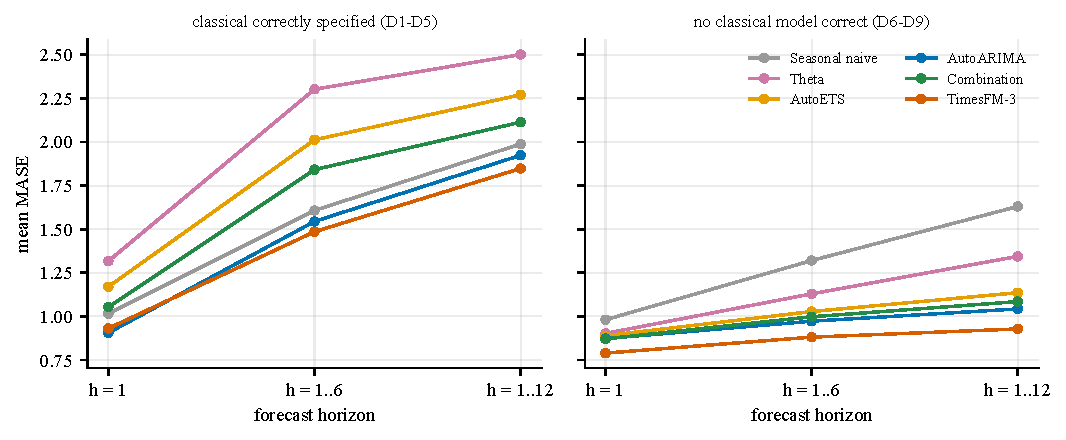
\includegraphics[width=\textwidth]{../figures/fig4_horizon.pdf}
\caption{Mean MASE by forecast horizon, averaged within each regime. Left: the five processes
for which a classical family is correctly specified. Right: the four for which none is. The
averages are dominated by the cells in which an automatic classical method fails badly, which is
why TimesFM-3 leads both panels even though the classical methods win more individual cells.}
\label{fig:horizon}
\end{figure}

\subsection{Coverage of prediction intervals}
\label{sec:coverage}

\begin{figure}[!htbp]
\centering
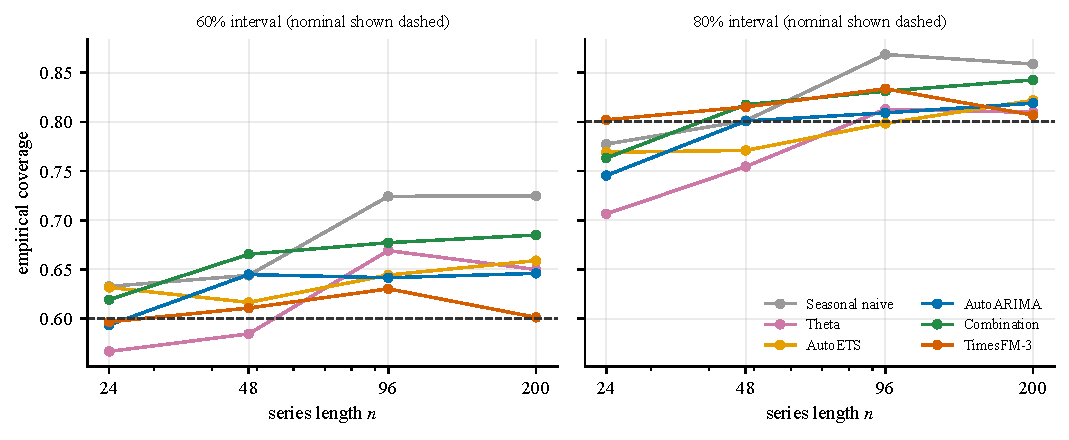
\includegraphics[width=\textwidth]{../figures/fig3_coverage.pdf}
\caption{Empirical coverage of the nominal 60\% and 80\% intervals, averaged over all nine
processes, against series length. The nominal level is dashed. TimesFM-3's 80\% coverage stays
within 0.802--0.834 across every length; the classical methods under-cover at $n = 24$ and
over-cover from $n = 96$.}
\label{fig:coverage}
\end{figure}

\figureref{fig:coverage} reports empirical coverage against nominal, averaged over the nine
processes. On that averaged view TimesFM-3's 80\% coverage stays between 0.802 and 0.834 across
series lengths, closer to nominal than any other method, while seasonal naive drifts from 0.777
at $n = 24$ to 0.869 at $n = 96$.

The averaged view nevertheless understates the typical deviation from nominal coverage for
every method. Averaging coverage across processes lets over-coverage on one process cancel
under-coverage on another, so the deviation of an average understates the typical error. The
appropriate statistic is the mean of the per-cell absolute deviations, and it is roughly three
times larger: 0.047 for TimesFM-3, 0.066 for AutoARIMA, 0.089 for the combination, 0.101 for
AutoETS, 0.127 for Theta and 0.144 for seasonal naive. The ranking is unchanged and TimesFM-3
remains the best calibrated, but the level is not close to nominal: \textbf{its per-cell 80\%
coverage ranges from 0.583 to 0.921}. No method in this study delivers reliable 80\% intervals
across all nine processes. This divergence is expected by construction: classical prediction intervals rely on an assumption of
Gaussian innovations $\mathcal{N}(0, \sigma^2)$, which is violated by design on the intermittent
process D8 (Poisson arrivals) and the GARCH process D9 (heavy-tailed innovations with time-varying volatility).
While an analyst could specify custom non-Gaussian likelihoods or bootstrapped intervals, applied practitioners
predominantly rely on automated software defaults; evaluating standard classical intervals against the
learned quantile head of TimesFM-3 thus highlights the practical operational consequences of that misspecification in automated workflows.

The structural-break process D6 is the sharpest illustration, and it shows why coverage alone
is a misleading summary. Every classical method covers between 0.966 and 0.999 there against a
nominal 0.80. This over-coverage is a symptom of misspecification rather than evidence of reliability. The break inflates the estimated
innovation variance, so the intervals become enormous---scaled widths of 4.8 to 10.4, against
3.0 to 5.1 for TimesFM-3. The classical intervals contain the truth almost always because they
contain almost everything. TimesFM-3 covers between 0.828 and 0.889, still above nominal, using
intervals roughly half as wide.

\subsection{Robustness to the combination rule}
\label{sec:combination}

TimesFM-3 beats the pre-registered equal-weight combination in 27 of 30 significant
comparisons, which invites the objection that the combination was weak---it contains Theta,
which fails badly in several cells, and a mean is not robust to one broken member. The comparison
was therefore repeated against a \emph{median} combination of the same three methods. The
objection does not hold: the median combination is slightly worse than the mean combination
(mean MASE 1.712 against 1.656, with TimesFM-3 at 1.439), and TimesFM-3 still wins 25 of 29
significant comparisons. The median rule gains robustness at the cost of the averaging that
motivates combination: with three members, the median is the middle of the three forecasts at
each time point, so it forgoes the cancellation of errors from which the mean combination
benefits, and the mean combination is more accurate than the average of its members in all 36
cells. This analysis is post hoc and is reported as such.

\subsection{Undefined values of MAPE}
\label{sec:mape}

MAPE is undefined for 12\,906 of the 129\,600 evaluations---9.96\%, and every one of
them on the intermittent process D8. A study that had used MAPE as its headline metric would
have had to drop the single regime in which TimesFM-3 wins most decisively, or silently
substitute a convention for the zeros. This illustrates a well-known limitation of the measure
\citep{hyndman2006mase, kolassa2016count}, and it is why MAPE appears here only in
\appendixref{app:mape}.

\section{Representativeness and robustness of the design}
\label{sec:robustness}

The conclusions of any simulation study are conditional on the processes and parameter values it
uses. This section asks two questions of the design in \sectionref{sec:design}: how closely the
simulated series resemble real series (\sectionref{sec:representativeness}), and whether the
headline conclusions survive when the parameters are drawn at random and the assumptions of
Gaussian, outlier-free data with a known seasonal period are relaxed
(\sectionref{sec:departures}). Both analyses were added after the main results were available and
are reported as post hoc; the pre-registered comparison is that of \sectionref{sec:results}.

\subsection{Representativeness of the simulated series}
\label{sec:representativeness}

Following \citet{kang2017instance}, every series is summarised by four features: the normalised
spectral entropy, a measure of forecastability equal to one for white noise; the strength of
trend and the strength of seasonality from an STL decomposition with period 12; and the
first-order autocorrelation of the first differences. The simulated series at $n = 96$ are placed
in this feature space together with the 1\,000 M4 Monthly series of \sectionref{sec:realdata},
each cut to its last 96 observations so that all series have the same length. An M4 series is
counted as \emph{covered} when some simulated series lies at least as close to it, in standardised
feature space, as the 95th percentile of the distance from an M4 series to its nearest other M4
series.

\figureref{fig:instance} shows the first two principal components of the feature space. The
fixed-parameter design of \tableref{tab:dgps} covers 56\% of the M4 series. Its processes form
compact clusters, because each uses a single parameter vector, and the regions between the
clusters, which contain many real series, are empty. The randomised-parameter design described in
\sectionref{sec:departures} covers 81\%. The M4 series lie closest to the trending processes: their
median trend strength is 0.88, against 0.63 for the simulated series. Almost none of them
(1\%) lies nearest to the intermittent process D8, because M4 contains no intermittent series; the
intermittent-demand results therefore rest on the simulation alone and on the literature for
that regime \citep{syntetos2005categorization}.

\begin{figure}[!htbp]
\centering
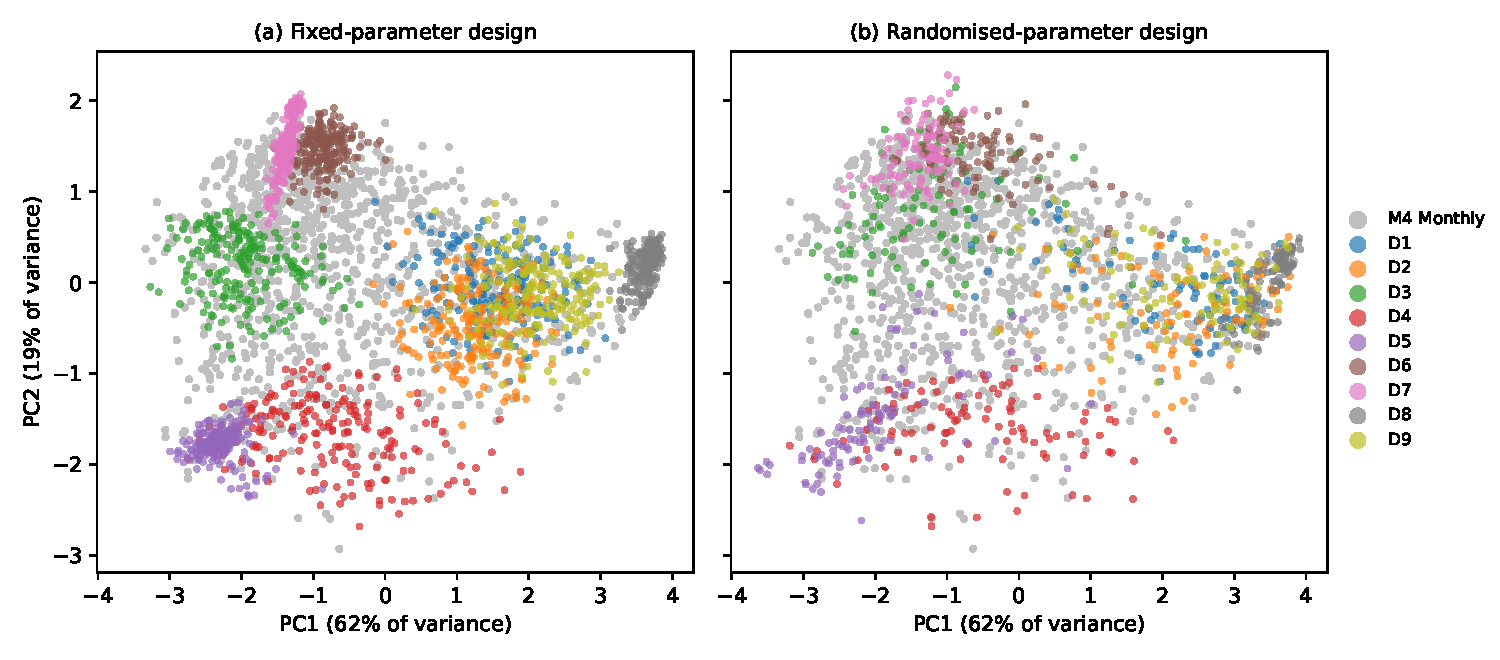
\includegraphics[width=\textwidth]{../figures/fig11_instance_space.pdf}
\caption{Simulated and M4 Monthly series in a four-feature instance space (spectral entropy,
trend strength, seasonal strength and first-order autocorrelation of the differences), first two
principal components. Grey points are M4 series; coloured points are simulated series at
$n = 96$. The share of M4 series covered is defined in \sectionref{sec:representativeness}.}
\label{fig:instance}
\end{figure}

\subsection{Randomised parameters and departures from the assumptions}
\label{sec:departures}

In the second analysis every series draws its own parameter vector uniformly from the ranges in
\tableref{tab:ranges}, each of which contains the fixed value of \tableref{tab:dgps}. The ranges
extend the linear processes towards the stationarity boundary ($\phi$ up to 0.95), cover
intermittency from lumpy ($p = 0.1$) to nearly continuous ($p = 0.6$) demand, and include breaks
from three to fifteen noise standard deviations in either direction. Four versions of the design
are run on the same 3\,600 parameter draws (100 per process and length):

\begin{itemize}
\item \emph{random parameters}: Gaussian innovations, as in the main design;
\item \emph{heavy tails}: Student-$t$ innovations with three degrees of freedom, rescaled to the
      same variance; for D8, negative binomial demand sizes with the same mean and three times
      the Poisson variance;
\item \emph{outliers}: each observation of the context is shifted, with probability 0.03, by four
      to six robust standard deviations in a random direction (for D8, a demand is multiplied by
      five), while the held-out values are left uncontaminated;
\item \emph{estimated period}: the series of the first version, but the classical methods receive
      the seasonal period selected by the 90\% autocorrelation test used for the M4 benchmarks
      \citep{makridakis2020m4}, applied when at least three cycles are observed, instead of the
      true one. This removes the classical methods'
      oracle knowledge of the period (\sectionref{sec:methods}); TimesFM-3 never receives a
      period, so its forecasts are unchanged.
\end{itemize}

\begin{table}[!htbp]
\centering
\begin{threeparttable}
\caption{Parameter ranges of the randomised-parameter design.}
\label{tab:ranges}
\small\setlength{\tabcolsep}{4pt}
\begin{tabular}{ll}
\toprule
ID & Parameters, each drawn uniformly on the stated interval \\
\midrule
D1 & $\phi \in [0.10, 0.95]$, $\sigma \in [1, 5]$ \\
D2 & $\phi \in [0.10, 0.90]$, $\theta \in [-0.6, 0.8]$, $\sigma \in [1, 5]$ \\
D3 & $\phi \in [-0.5, 0.8]$, $\theta \in [-0.5, 0.6]$, drift $\in [0, 0.6]$, $\sigma \in [1, 5]$ \\
D4 & $\phi \in [0.1, 0.8]$, $\Phi \in [0.1, 0.8]$, seasonal amplitude $\in [5, 20]$, $\sigma \in [1, 5]$ \\
D5 & $\alpha \in [0.05, 0.5]$, $\beta \in [0.001, 0.03]$, $\gamma \in [0.05, 0.3]$, initial trend $\in [0, 0.5]$, amplitude $\in [5, 20]$ \\
D6 & jump $\in [3, 15]\,\sigma$ with random sign, break at $[0.50, 0.85]\,n$, level noise $\in [0.2, 1]$ \\
D7 & $r \in [0.04, 0.15]$, inflection at $[0.4, 0.8](n + H)$, $K \in [100, 250]$, $\sigma \in [1, 6]$ \\
D8 & demand probability $p \in [0.1, 0.6]$, size $1 + \mathrm{Pois}(\lambda)$ with $\lambda \in [1, 8]$ \\
D9 & $\phi \in [0.1, 0.9]$, $a \in [0.05, 0.15]$, $b \in [0.75, 0.90]$, with $a + b < 0.98$ \\
\bottomrule
\end{tabular}
\begin{tablenotes}[flushleft]\footnotesize
\item \textit{Note:} Parameters not listed are as in \tableref{tab:dgps}. The intervals contain the
fixed values of the main design. Seeds are disjoint from those of the main design, and the four
versions use the same parameter draws and innovations, so they are paired.
\end{tablenotes}
\end{threeparttable}
\end{table}

\begin{table}[!htbp]
\centering
\begin{threeparttable}
\caption{Headline conclusions under randomised parameters and departures from the assumptions.}
\label{tab:robust-design}
\small\setlength{\tabcolsep}{4pt}
\begin{tabular}{lcccc}
\toprule
 & Random & Heavy tails & Outliers & Tested seas. \\
\midrule
TimesFM-3 cell wins (of 36) & 14 & 15 & 16 & 16 \\
TimesFM-3 median ratio to cell-best & 1.029 & 1.038 & 1.004 & 1.017 \\
TimesFM-3 worst ratio to cell-best & 1.56 & 1.54 & 1.49 & 1.55 \\
Smallest worst ratio, classical & 2.12 & 2.32 & 2.09 & 1.58 \\
Significant comparisons, won--lost & 93--29 & 100--28 & 101--27 & 100--27 \\
D4, $n \geq 48$: AutoARIMA better (of 3) & 3 & 3 & 2 & 3 \\
D8: Croston better on RMSSE (of 4) & 4 & 4 & 4 & 4 \\
D5, $n = 24$: AutoETS / seasonal naive ($m = 12$) & 2.03 & 2.05 & 1.91 & 2.25 \\
\bottomrule
\end{tabular}
\begin{tablenotes}[flushleft]\footnotesize
\item \textit{Note:} 200 replications per (process, length) cell, 7\,200 series per column; every series draws its own parameters from the ranges in Table~S8 of the Supporting Information. Ratios use mean MASE over $h = 1, \dots, 12$. Significant comparisons are paired Wilcoxon tests of TimesFM-3 against each of the five general-purpose classical methods in each cell (180 per column), Benjamini--Hochberg at 0.05 within each (column, opponent) family of 36 cells (the main design's families also include the three horizon slices). The D8 row compares TimesFM-3 with the best of Croston-SBA, TSB and ADIDA; the last row divides by seasonal naive with the true period in every column. In the tested-seasonality column the classical methods use $m = 12$ only where the M4 seasonality test finds seasonality; TimesFM-3's forecasts are those of the first column.
\end{tablenotes}
\end{threeparttable}
\end{table}


\tableref{tab:robust-design} checks the headline conclusions of \sectionref{sec:results} in each
version. Four of them hold in every version, one of them in weakened form when the context
contains outliers.

\begin{itemize}
\item \emph{Robustness rather than peak accuracy.} TimesFM-3 is the best method in 13 to 18 of the
      36 cells and within 3.2\% of the cell-best method in the median cell. Its worst ratio to the
      cell-best rises from 1.31 in the fixed design to between 1.45 and 1.51, and the worst cells
      are now on the logistic process D7, where the equal-weight combination is best. Every
      classical method remains worse than this somewhere: the smallest worst ratio among them is
      2.16 to 2.29, and 1.60 when the period is estimated.
\item \emph{Pairwise comparisons.} TimesFM-3 wins 78 to 89 of the 180 comparisons in each version
      and loses 16 to 20, close to the proportions of the main design. AutoARIMA again remains
      the classical method against which it has the fewest wins (6--5, 6--6, 10--3 and 7--4 in
      the four versions).
\item \emph{Intermittent demand.} TimesFM-3 has a lower MASE than the best Croston-family method
      at every length in three versions, and at three of four lengths with outliers, while the
      Croston family has the lower RMSSE at every length in all four. The reversal between the two
      error measures therefore holds across the parameter range examined, not only at one value.
\item \emph{Seasonality with enough cycles.} AutoARIMA is more accurate than TimesFM-3 on D4 at
      every length from $n = 48$ in three versions, by a median of 20--26\%. With outliers, it is
      better at two of three lengths and by only 6\%, since outliers in the context disturb the
      estimation of the seasonal model more than they disturb TimesFM-3.
\end{itemize}

The fifth conclusion, the collapse of correctly specified exponential smoothing when only two
seasonal cycles are observed, is qualified. With Gaussian, heavy-tailed or contaminated innovations AutoETS has 1.96 to 2.14 times
the mean MASE of seasonal naive on D5 at $n = 24$, against 2.7 in the fixed design, so the effect
persists at a smaller size. When the period is estimated, however, the ratio falls to 1.00: the
seasonality test is applied only when at least three full cycles are observed, so at
$n = 24$ every series is treated as
non-seasonal and no seasonal model is fitted. The failure is therefore caused by forcing a
seasonal model onto two cycles, which is the estimability explanation of
\sectionref{sec:estimability}; a practitioner who applies a standard seasonality test avoids it.

\figureref{fig:response} shows how the relative accuracy of TimesFM-3 and AutoARIMA depends on
the drawn parameters. It is flat in the autoregressive coefficient of D1 and the GARCH
persistence of D9, so the conclusions for those processes do not depend on the fixed values
chosen in \tableref{tab:dgps}. It moves strongly with the demand probability of D8: at $p$ near
0.15 TimesFM-3 has about 40--50\% lower MASE than AutoARIMA, and the advantage disappears as $p$
approaches 0.5, where demand is no longer intermittent. On D6 the advantage of TimesFM-3 grows
with the size of the break, and on D7 the comparison changes sign with the position of the
inflection point, which is consistent with the dependence on series length found for that
process in the main design.

\begin{figure}[!htbp]
\centering
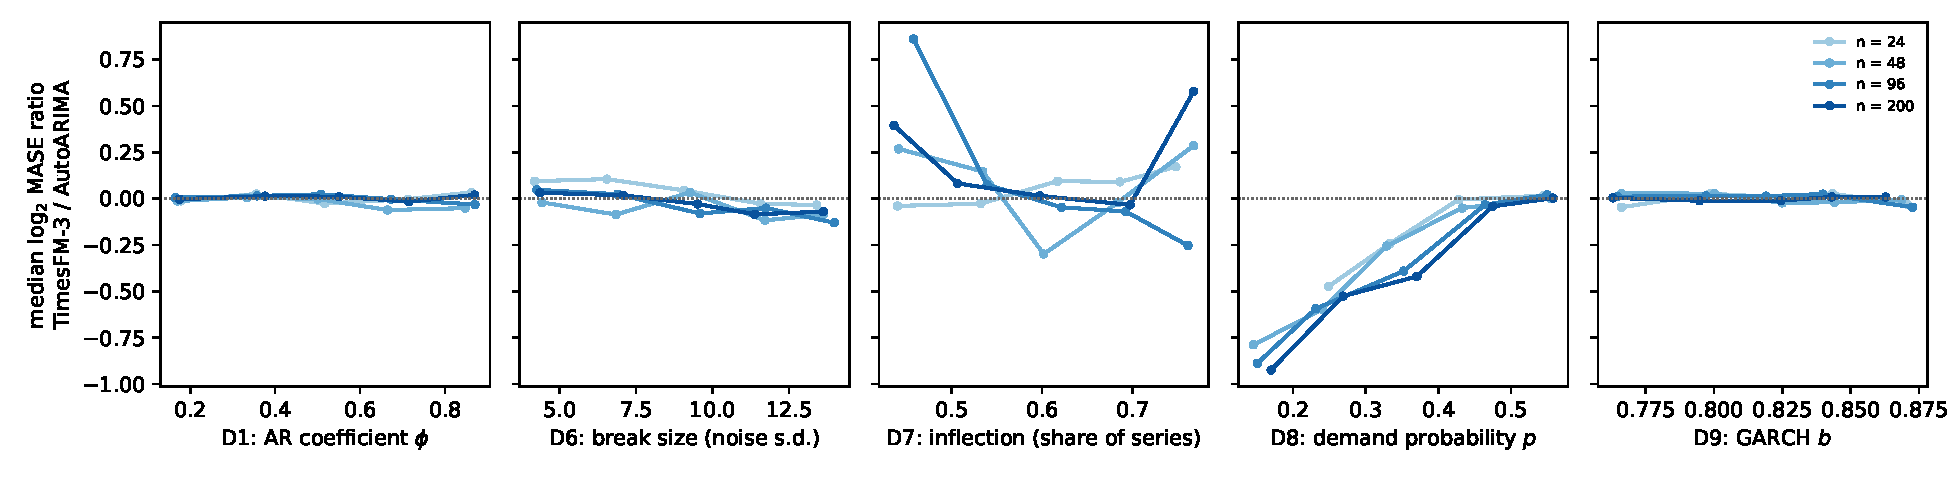
\includegraphics[width=\textwidth]{../figures/fig12_parameter_response.pdf}
\caption{Median $\log_2$ ratio of the MASE of TimesFM-3 to that of AutoARIMA, by quintile of the
drawn parameter, randomised-parameter design with Gaussian innovations. Values below zero favour
TimesFM-3.}
\label{fig:response}
\end{figure}

\section{Application to M4 monthly data}
\label{sec:realdata}

The simulation tier secures freedom from contamination at the cost of realism. This section
complements it with real data, subject to an important caveat: \textbf{the M4 data may be
contaminated}. M4 is a widely used public benchmark and is likely to be contained in TimesFM-3's
pre-training corpus \citep{meyer2025leakage}, so an advantage of TimesFM-3 here may reflect
memorisation rather than forecasting skill; for this reason the simulation tier carries the
primary claim. The real-data tier addresses a narrower question, namely which of the simulated
regimes real monthly series resemble. \sectionref{sec:m4design} describes the sampling and
evaluation design, and \sectionref{sec:m4results} reports the results.

\subsection{Sampling and evaluation design}
\label{sec:m4design}

A seeded random sample of 1\,000 series is drawn from the 32\,581 M4 monthly series long enough
for the design, and each series is evaluated at three rolling origins spaced 12 months apart with M4's own
monthly horizon, $h = 18$. Three origins per series would give 3\,000 windows; the realised
count is 2\,932, because a series shorter than 138 observations cannot support the third
origin once 18 held-out points and a 120-observation minimum context are subtracted, and those
68 windows are dropped rather than shortened. The sampled series are substantial: median
length 299 observations, upper quartile 324, maximum 1\,808.

The pre-registered protocol specified the Diebold--Mariano test here. With only three origins per
series that statistic carries two degrees of freedom and has essentially no power, so the analysis
is instead a paired Wilcoxon test across the 1\,000 series---which are independent units, unlike
the overlapping windows within a series. Diebold--Mariano is not reported at all; the reasons are
given in \sectionref{sec:evaluation} and the departure is recorded.

\subsection{Empirical results}
\label{sec:m4results}

\tableref{tab:realdata} gives the outcome, and it reproduces the simulation's pattern closely.
TimesFM-3 significantly outperforms seasonal naive (better on 80.1\% of series), Theta (56.8\%)
and AutoETS (54.1\%), and is \emph{statistically indistinguishable} from both AutoARIMA (52.6\%,
adjusted $p = 0.27$) and the combination (48.5\%, adjusted $p = 0.27$).

\begin{table}[!htbp]
\centering
\begin{threeparttable}
\caption{Comparison of TimesFM-3 with the classical methods on 1\,000 M4 monthly series.}
\label{tab:realdata}
\begin{tabular}{lrrrrl}
\toprule
Comparison & Mean MASE & Median ratio & \% series better & Adj.\ $p$ & Verdict \\
\midrule
TimesFM-3          & 0.914 & ---   & ---  & ---    & \\
\midrule
vs seasonal naive  & 1.280 & 0.699 & 80.1 & $<0.0001$ & TimesFM-3 \\
vs Theta           & 0.970 & 0.933 & 56.8 & $<0.0001$ & TimesFM-3 \\
vs AutoETS         & 0.951 & 0.966 & 54.1 & 0.0043    & TimesFM-3 \\
vs AutoARIMA       & 0.923 & 0.970 & 52.6 & 0.27      & tie \\
vs combination     & 0.907 & 0.996 & 48.5 & 0.27      & tie \\
\bottomrule
\end{tabular}
\begin{tablenotes}[flushleft]\footnotesize
\item \textit{Note:} Up to three rolling origins per series (2\,932 windows in all), $h = 18$.
Mean MASE is that of the method named in each row; a median ratio below 1 and a share of series
above 50\% favour TimesFM-3. Paired Wilcoxon tests across series, Benjamini--Hochberg corrected.
\end{tablenotes}
\end{threeparttable}
\end{table}

Two observations follow.

First, \textbf{the two tiers agree}. M4 Monthly series are long (median 299 observations) and
seasonal---precisely the regime in which the simulation found classical methods competitive or
better, because there is ample data with which to estimate the right model. Real monthly data
therefore fall in the estimable regime, and the real-data result is the one that
\sectionref{sec:results} predicts for that regime. The agreement is worth more than either tier alone, since the two have opposite
weaknesses.

Second, \textbf{the probabilistic results diverge}.
TimesFM-3's interval \emph{coverage} does not carry over: on simulated data it was the best
calibrated, whereas here it is the worst but one, covering 0.765 against a nominal 0.80 while the
combination achieves 0.801. Yet on the pre-registered proper scoring rule---the scaled pinball
loss over the nine deciles---TimesFM-3 is \textbf{the best of the six methods} (0.363, against
0.365 for the combination and 0.374 for AutoARIMA), even though the combination edges it on mean
MASE.

These are not in conflict; they measure different things. Coverage asks only whether the truth
falls inside one interval, and is blind to how the remaining probability mass is arranged; the
pinball loss scores the whole predictive distribution across all nine deciles. TimesFM-3's
distribution is therefore better \emph{overall} while its 80\% interval is too narrow. A reader
who cares about a calibrated interval should prefer the combination here; a reader who cares
about the full predictive distribution should prefer TimesFM-3. Reporting only the coverage
figure would have understated it, and reporting only the pinball loss would have overstated it.
The fragility of foundation-model calibration reported by \citet{adler2026calibrated} is visible
in the coverage half of this result.

\section{Operational considerations}
\label{sec:operational}

Accuracy is not the only criterion for choosing a forecasting method. This section considers four
further criteria: computational cost (\sectionref{sec:cost}), the licensing of model weights
(\sectionref{sec:licence}), interpretability and diagnostics (\sectionref{sec:interpret}), and
the theoretical basis of prediction intervals (\sectionref{sec:intervals}).

\subsection{Computational cost}
\label{sec:cost}

A 330-million-parameter network might be expected to be more expensive to run than a
statistical model with a handful of parameters. On the hardware used here, the reverse holds.
\tableref{tab:timing} reports each method timed separately on the same 200 series.

\begin{table}[!htbp]
\centering
\begin{threeparttable}
\caption{Wall-clock computing time per series.}
\label{tab:timing}
\begin{tabular}{lrr}
\toprule
Method & Time per series (ms) & Relative to TimesFM-3 \\
\midrule
Seasonal naive & 3.1 & $0.13\times$ \\
Theta & 9.0 & $0.39\times$ \\
\textbf{TimesFM-3} (GPU, batched) & \textbf{23.2} & $1\times$ \\
AutoETS & 102.0 & $4.4\times$ \\
\textbf{AutoARIMA} & \textbf{2382.7} & $\mathbf{102.8\times}$ \\
\bottomrule
\end{tabular}
\begin{tablenotes}[flushleft]\footnotesize
\item \textit{Note:} Each method timed separately on 200 seasonal series of length 96
($h = 12$). TimesFM-3 was run on an NVIDIA GTX 1660 Ti; its one-off model load of 3.0\,s is
excluded, as are the classical methods' import costs.
\end{tablenotes}
\end{threeparttable}
\end{table}

AutoARIMA is \textbf{103 times slower per series than TimesFM-3}. The reason is structural
rather than incidental: automatic ARIMA runs a stepwise search over model orders, fitting each
candidate by maximum likelihood, separately for every series. TimesFM-3 performs one batched
forward pass and amortises it across the batch. Where a practitioner's constraint is throughput
over many series---which is exactly the setting in which \sectionref{sec:results} found the
foundation model most attractive---the accuracy argument and the cost argument point the same
way.

Memory use was also pre-registered as an operational cost, but its measurement here is limited. Peak \proglang{Python} heap allocation during fitting was about 1\,MB
for every classical method (0.6\,MB for Theta, 1.4\,MB for AutoARIMA), but that instrument counts
only \proglang{Python}-level allocations and sees neither the compiled \pkg{numba} kernels the
classical methods run in nor the GPU memory TimesFM-3 uses, so no comparable figure for TimesFM-3
can be given. What can be said without measurement is structural: the classical methods hold a
handful of parameters per series, while TimesFM-3 requires its 330-million-parameter checkpoint
resident throughout---roughly 1.3\,GB---which is the binding memory constraint in any deployment
and is invariant to how many series are being forecast.

Two qualifications apply, and the second is more important than the per-series ratio.
TimesFM-3's figure depends on a GPU; without one the comparison narrows substantially. And the
classical methods parallelise trivially across series, which recovers most of the difference: in
the study's own main run, fitting all four classical methods over all 7\,200 series took 7.3
minutes on 22 cores, against 3.2 minutes for TimesFM-3 on a single consumer GPU---a ratio of
$2.3\times$, not $103\times$.

The per-series figure and the end-to-end figure answer different questions, and quoting only the
first would overstate the case. The fair summary is that TimesFM-3 is dramatically cheaper than
AutoARIMA per series on one core, and modestly cheaper than the whole classical suite once that
suite is given a 22-core machine. On none of the measures taken here is it the more expensive
option.

\subsection{Licensing of model weights}
\label{sec:licence}

The most consequential difference between the two families is not statistical. TimesFM-3's
pre-trained weights are released under \code{timesfm-non-commercial-license-v1.0} and are
restricted to non-commercial, non-production use \citep{timesfm3repo}. The source code remains
Apache-2.0, and so were the weights of TimesFM-2.5, but the version-3 weights are not.

This restriction takes precedence over any accuracy consideration: \textbf{for a
commercial forecasting application, TimesFM-3 as released is unavailable at any accuracy}. A
26\% MASE reduction on intermittent demand is irrelevant to a retailer who may not lawfully
deploy the model that achieves it. The available responses are to use TimesFM-2.5 under
Apache-2.0, to negotiate separate terms, or to use a classical method. Every classical method
compared here is free of such restrictions.

The point is noted because licensing is routinely omitted from model comparisons, although it
determines which models are admissible for an entire class of users.

\subsection{Interpretability and diagnostics}
\label{sec:interpret}

An ARIMA fit reports its orders, its coefficients and their standard errors; an ETS fit reports
its smoothing parameters and states. These support the ordinary diagnostic work of applied
forecasting---inspecting residuals, testing for remaining autocorrelation, explaining to a
stakeholder why the forecast turns where it does, and detecting when a model has stopped
fitting. TimesFM-3 exposes none of this. When it forecasts poorly there is no parameter to
inspect and no diagnostic to run; the available response is to notice the errors and switch
methods. In regulated settings where a forecast must be justified rather than merely produced,
this difference may outweigh the accuracy comparison entirely.

\subsection{Theoretical basis of prediction intervals}
\label{sec:intervals}

The classical intervals derive from a model's assumed error structure and can be reasoned about
analytically. TimesFM-3's quantiles are learned outputs of a network head, with no accompanying
theory. \sectionref{sec:coverage} shows that the learned quantiles are better calibrated on
average, but this holds empirically for these processes rather than by construction, and their
behaviour on a process unlike anything in the pre-training corpus is unknown.

\section{Discussion}
\label{sec:discussion}

This section assesses the pre-registered hypotheses (\sectionref{sec:hypotheses}), interprets the
balance between robustness and peak accuracy (\sectionref{sec:tradeoff}), translates the evidence
into practical recommendations (\sectionref{sec:recommendations}), and states the limitations of
the study (\sectionref{sec:limitations}).

\subsection{Assessment of the pre-registered hypotheses}
\label{sec:hypotheses}

Of the five pre-registered hypotheses, \textbf{none survives unqualified}: two are refuted
outright, two are partially supported, and one is refuted in its second clause.

\begin{itemize}
\item \textbf{H1} (correctly specified classical models beat TimesFM-3 on their home ground,
      gap largest at short lengths) --- \textbf{refuted as stated}. The gap at short lengths runs
      the other way. What survives is narrower: where a classical model is both correctly
      specified \emph{and} estimable, it wins (D4 and D5 at $n \geq 48$).
\item \textbf{H2} (TimesFM-3 wins wherever no classical form is correct) ---
      \textbf{partially supported}. It holds on intermittent demand under MASE and pinball loss
      but not under RMSSE or sMAPE, mildly on structural breaks, and not on the logistic process,
      where the outcome depends on length.
\item \textbf{H3} (on D9 the families are indistinguishable in the mean, classical intervals
      under-cover) --- \textbf{partially supported}. The families are indeed indistinguishable in
      the mean, but AutoARIMA is the only classical method that under-covers on D9; the others
      over-cover.
\item \textbf{H4} (the combination beats every individual classical method and is the hardest
      baseline for TimesFM-3) --- \textbf{refuted in both clauses}. AutoARIMA beats the
      combination on mean MASE, and AutoARIMA, not the combination, is the baseline TimesFM-3
      finds hardest (11--9, against 27--3 for the combination).
\item \textbf{H5} (both families under-cover at 80\%) --- \textbf{refuted}. On the
      process-averaged view TimesFM-3 sits close to nominal and the classical methods over-cover
      from $n = 96$; on the per-cell view every method's typical deviation is far larger
      than expected, but not systematically downward.
\end{itemize}

That every hypothesis failed in some respect illustrates the value of pre-registration: the
hypotheses were stated before any result was available and are assessed here as they were stated.

\subsection{Robustness versus peak accuracy}
\label{sec:tradeoff}

A count of 16 cell wins against 20 might be read as evidence that the classical methods remain
superior. That reading overlooks the fact that the 20 wins are distributed across five different
methods: AutoARIMA 10, seasonal naive 4, and two each for the others. The classical column of
\tableref{tab:mase} is a column of \emph{different} winners, and which one wins is not knowable
in advance without the kind of model-selection work the foundation model is meant to remove.
TimesFM-3, one model with no tuning, is within noise of that per-cell best in half the design
and beaten decisively in only two regimes.

The evidence therefore supports neither the conclusion that foundation models have superseded
classical methods nor the conclusion that classical methods remain superior. It supports a
narrower conclusion: \textbf{TimesFM-3 provides robustness rather than peak accuracy}, and
\tableref{tab:robust} puts a number on the trade: it is within 0.8\% of the cell-best method in
the median cell and never more than $1.31\times$ worse anywhere, while every classical method is
somewhere at least $2.2\times$ worse. In this design it is rarely the best method and never among
the worst, whereas
the automatic classical methods are sometimes excellent and sometimes catastrophic---AutoETS at
3.03 on data generated by an ETS process is the cautionary example. For a forecaster with one
well-understood series, that trade is unattractive. For a forecaster with ten thousand
heterogeneous series and no capacity to diagnose each one, the trade favoured TimesFM-3 in this
design, because its worst case was much milder than that of any classical method.

\subsection{Practical recommendations}
\label{sec:recommendations}

\tableref{tab:decision} translates the evidence into recommendations. They are deliberately
narrow: they apply strictly to the regimes examined, and they name more than one option wherever the
evidence does not support a single preference. Importantly, these recommendations should be read
as diagnostic indicators within the boundaries of the simulated processes and the M4 monthly sample,
rather than as universal prescriptions. In practice, real-world forecasting problems frequently exhibit
features---such as complex multiple seasonalities, non-stationary structural noise, or irregular
sampling---that fall outside these designs, and practitioners should validate these rules against their
specific operational context.

\begin{table}[!htbp]
\centering
\begin{threeparttable}
\caption{Recommended forecasting family by situation, within the regimes examined.}
\label{tab:decision}
\small
\begin{tabular}{>{\raggedright\arraybackslash}p{5.5cm}>{\raggedright\arraybackslash}p{3.0cm}>{\raggedright\arraybackslash}p{5.0cm}}
\toprule
Situation & Use & Evidence \\
\midrule
Commercial or production deployment
  & Classical (or TimesFM-2.5)
  & Version-3 weights are licensed non-commercial; accuracy is not the binding constraint \\[2pt]
Intermittent demand, and the decision loss is roughly linear in units
  & \textbf{TimesFM-3}, but see the caveat
  & Beats all six Croston-family methods on MASE at every length (24/24 significant), and the
    general-purpose set by 22--26\%, but worse on RMSSE and sMAPE (D8) \\[2pt]
Intermittent demand, and the decision loss is roughly quadratic
  & Classical
  & The metrics reverse: Croston-SBA and ADIDA win on RMSSE at every length (D8) \\[2pt]
Strong seasonality, at least four full cycles observed
  & \textbf{AutoARIMA}
  & AutoARIMA 21--24\% better; TimesFM-3 27--31\% worse, all $p < 0.0001$ (D4).
    Reverses below four cycles \\[2pt]
Short series with seasonality (two cycles or fewer)
  & Seasonal naive or TimesFM-3
  & Automatic classical methods fail badly here: AutoETS scores 3.03 on its own process (D5, $n=24$) \\[2pt]
Many heterogeneous series, no capacity to select and tune a model per series
  & \textbf{TimesFM-3}
  & Beats every classical method except AutoARIMA in the large majority of significant comparisons \\[2pt]
One series, and you can identify and estimate the right model
  & Classical
  & AutoARIMA and TimesFM-3 are close (11--9 significant comparisons); AutoARIMA is free to use, interpretable and diagnosable \\[2pt]
Structural break in the recent past, intervals matter
  & \textbf{TimesFM-3}
  & Comparable coverage using intervals roughly half as wide (D6, simulation only) \\[2pt]
Throughput matters and a GPU is available
  & \textbf{TimesFM-3}
  & 103$\times$ faster per series than AutoARIMA; $2.3\times$ faster than the whole
    classical suite on 22 cores \\[2pt]
Well-calibrated intervals on real data are the priority
  & Classical combination
  & On M4 the combination covered 0.801 against nominal 0.80; TimesFM-3 under-covered at
    0.765 \\[2pt]
The forecast must be explained or audited
  & Classical
  & TimesFM-3 exposes no parameters, residual diagnostics or interval theory \\
\bottomrule
\end{tabular}
\begin{tablenotes}[flushleft]\footnotesize
\item \textit{Note:} Based on the evidence in Sections~\ref{sec:results}--\ref{sec:operational}.
Bold marks a preference supported by significant differences; the remaining rows rest on
considerations outside the accuracy comparison.
\end{tablenotes}
\end{threeparttable}
\end{table}

\subsection{Limitations}
\label{sec:limitations}

Seven limitations bound these conclusions.

First, the simulation tier's strength is also its boundary. Series generated from nine
parametric processes are not real series; they are clean, stationary where specified, and free
of the measurement error, calendar effects, promotions and regime changes that characterise
applied work. What the simulation buys---provable absence of contamination and known correct
specification---it pays for in realism, which is why \sectionref{sec:realdata} exists.

Second, TimesFM-3 was evaluated zero-shot and univariate. Its headline novelty is native
multivariate forecasting with covariates, and that capability is untested here because the
simulated processes are univariate by construction. A study exercising cross-series information
could reach different conclusions, and would be the natural sequel.

Third, no method received hand-tuning. That is deliberate and it is the comparison most
practitioners face, but an expert who identified each process by eye and fitted the
corresponding model by hand would beat every automatic method reported here, including on D4
and D5 at $n = 24$.

Fourth, the horizon is short ($H = 12$) and the seasonal period fixed at 12. Longer horizons
and other frequencies may behave differently, and the calibration literature reports that
foundation-model calibration degrades with horizon \citep{adler2026calibrated}.

Fifth, the intermittent-demand analysis of \sectionref{sec:croston} is post hoc: the
Croston-family baselines were added after the main results were seen, in response to an
identified gap, and are reported separately from the pre-registered comparison.

Sixth, this study evaluates a single foundation model architecture: Google's TimesFM-3, a
decoder-only transformer operating on continuous, patched representations. Other architectures---such
as tokenized language models (e.g., Chronos; \citealp{ansari2024chronos}) or masked encoder-decoder
networks (e.g., MOIRAI; \citealp{woo2024moirai})---possess distinct inductive biases, loss functions,
and pre-training mixtures. Whether the robustness-versus-peak-accuracy trade-off documented here
holds across alternative foundation-model families remains an open question for multi-architecture comparisons.

Seventh, although \sectionref{sec:robustness} draws the parameters at random and relaxes three
assumptions, the processes themselves are fixed: nine univariate families at a single seasonal
period. The randomised design covers 81\% of the M4 monthly series in a four-feature space, which
leaves a fifth of real monthly series, and all series at other frequencies, outside the regions
studied. Coverage in four features is also a necessary rather than a sufficient condition for
similarity, since two series can share these features and differ in others.

\section{Conclusion}
\label{sec:conclusion}

This study compared TimesFM-3 with five classical alternatives on 7\,200 series generated from nine
known processes, under a pre-registered protocol, in a design where contamination of the
foundation model is impossible by construction and the classical models are correctly specified
by construction.

Neither family dominates. TimesFM-3 wins 16 of 36 cells and the classical methods 20, but the
20 are spread across five different winners while TimesFM-3 is a single untuned model. Against
individual classical methods it wins 113 of 132 significant comparisons, and only AutoARIMA
holds its own at 11--9. Measured against the best method in each cell, TimesFM-3 is never more
than $1.31\times$ worse anywhere in the design and is within 0.8\% of the best in the median
cell, while every classical method is somewhere at least $2.2\times$ worse. On strongly seasonal
data with at least four observed cycles AutoARIMA is 21--24\% better. On intermittent demand the
answer depends on the loss function: TimesFM-3 is about a quarter better on MASE and best on the
scaled pinball loss, but worse on RMSSE and much worse on sMAPE, because absolute- and
squared-error metrics reward different functionals of a predictive distribution that is 70\%
zeros.

These conclusions do not rest on the particular parameter values of the main design. When every
series draws its own parameters from wide ranges, and when the data have heavy-tailed noise,
outliers or a seasonal period that the classical methods must estimate, the same pattern holds:
TimesFM-3 is at most 1.51 times worse than the best method in any cell, the seasonal advantage of
AutoARIMA and the reversal between error measures on intermittent demand persist, and the collapse
of seasonal models on two cycles disappears once a standard seasonality test is applied. The
randomised design is also closer to real data, covering 81\% of M4 monthly series in a feature
space against 56\% for the fixed design.

A secondary analysis of 1\,000 M4 Monthly series reproduces the pattern closely: TimesFM-3 beats
seasonal naive, Theta and AutoETS significantly, and ties with AutoARIMA and the combination.
Real monthly series are long and seasonal---the estimable regime---and the tiers agree on what
happens there, which is worth more than either tier alone given their opposite weaknesses.

The finding most likely to transfer beyond this design concerns the classical side, where the
mechanism can be examined: the decisive property is not whether a classical model is correctly
\emph{specified} but whether it is \emph{estimable}. With two seasonal cycles, AutoETS had a mean
MASE 2.7 times that of the seasonal naive method on data generated by an ETS process. In this
design TimesFM-3 was most useful relative to the classical methods where classical estimation was
starved, and least useful where it was comfortable; whether the same holds for other foundation
models is not tested here.

Two findings outside the accuracy comparison deserve equal weight. TimesFM-3 is 103 times
faster per series than AutoARIMA, so the foundation model is the less expensive option per series,
although parallelising the classical suite across 22 cores narrows the end-to-end difference to
$2.3\times$. And its released weights may not be used commercially. For commercial applications,
this restriction takes precedence over the accuracy comparison.

Finally, the study is exploratory. It describes how one black-box model behaves on data of
known structure; it does not explain that behaviour, and its conclusions remain conditional on the
processes, parameter ranges and monthly horizons examined, even after the robustness analysis. A
simulation with a known ground truth and a pre-registered analysis can make such a description
reliable, but no synthetic design spans the heterogeneity of applied forecasting. Studies of other
foundation models, other sampling frequencies and multivariate problems with exogenous
regressors, and work on the internal representations of these models, will be needed before the
boundary between learned and parametric forecasting can be stated in general terms.

\section{Computational details and reproducibility}
\label{sec:repro}

All results were produced with \proglang{Python}~3.13 \citep{python}, using
\pkg{statsforecast}~2.1.1 \citep{statsforecast} for the classical methods and
\pkg{timesfm}~3.0.1 with the \path{google/timesfm-3.0-pytorch} weights \citep{timesfm3repo}
on \pkg{PyTorch}~2.6 \citep{paszke2019pytorch}. The simulation, evaluation and figures rest on
\pkg{NumPy} \citep{harris2020numpy}, \pkg{pandas} \citep{mckinney2010pandas}, \pkg{SciPy}
\citep{virtanen2020scipy} and \pkg{Matplotlib} \citep{hunter2007matplotlib}. Timings were taken
on an NVIDIA GTX 1660 Ti with a 24-core CPU and 32\,GB of memory; the loaded TimesFM-3
checkpoint reports 330\,710\,976 parameters.

Every simulated series is seeded deterministically from its own identifiers---process, length
and replication---so the entire study regenerates exactly from the code, independently of core
count or execution order. The analysis pipeline is split into cached phases, so each stage can
be re-run alone and the results reproduced without repeating the whole computation. The
robustness study of \sectionref{sec:robustness} uses a separate seed range and adds 91\,200
per-series evaluations; it ran in 42 minutes on the same machine, and its per-series metrics,
including every drawn parameter vector, are part of the archive.

Three aspects of research practice bear on the weight the results can carry. The protocol, including the five hypotheses, was frozen before any
forecast was produced, and the frozen file was never edited afterwards; nine departures from it
are recorded separately, each dated and reasoned, with the two post-hoc analyses marked as such.
Every DOI in the bibliography was resolved through \code{doi.org} content negotiation and its
record compared with the entry, and works published at venues that issue no DOI are cited by
their proceedings URL, with the preprint identifier given in a note. Finally, the hypotheses
refuted by the data (two outright and one in its stated form) are reported in \sectionref{sec:hypotheses} with the same prominence as those
that were partially supported.

\section*{Acknowledgements}

First and foremost, the authors thank Allah, the Almighty, for everything He has given them,
including the ability to complete this work.

The authors used a large language model solely to improve the language and readability of this
manuscript and to assist with the implementation of the simulation code. The authors reviewed and
edited all content and take full responsibility for the content of this publication.

\section*{Data and code availability}

The complete research compendium is archived on Zenodo at \code{10.5281/zenodo.22681072} (concept DOI, resolving to all versions): the pre-registered protocol, the deviation log, the entire pipeline, the per-series metrics for all 129\,600 evaluations, the raw forecasts and quantiles, every figure and the manuscript source. All data in the simulation tier are generated by that code from documented seeds; the real-data tier uses the publicly available M4 competition data \citep{makridakis2020m4}, which the code re-fetches, with the seeded 1\,000-series sample included so the analysis reproduces exactly.

The raw forecasts are deposited deliberately and not only for completeness. This paper's
intermittent-demand result reverses between absolute- and squared-error metrics, so a reader who
wants to re-score the same forecasts under a different loss can do so without re-running the
study. TimesFM-3's weights are not redistributed: they are released by Google under a
non-commercial licence and are downloaded by the code from Hugging Face.

\bibliographystyle{plainnat}
\bibliography{refs}

\newpage
\appendix

\section{Results under the mean absolute percentage error}
\label{app:mape}

\tableref{tab:mape} reports mean MAPE by process, alongside the percentage of series on which
it cannot be computed. The D8 row illustrates the problem: every intermittent series contains a zero,
so MAPE is undefined for all of them, and the process on which TimesFM-3 achieves its largest
and most consistent advantage simply drops out of the comparison.

The rankings also move. On D4, MAPE places seasonal naive first (2.360) and TimesFM-3 second
(2.801), whereas MASE places AutoARIMA first at every length from $n = 48$. MAPE's asymmetry
between over- and under-forecasts is enough to reorder the methods on the same forecasts.

% generated by code/09_make_tables.py -- do not edit by hand
\begin{table}[!htbp]
\centering
\begin{threeparttable}
\caption{Mean MAPE over $h = 1,\dots,12$ and percentage of series on which MAPE is undefined.}
\label{tab:mape}
\small
\begin{tabular}{lrrrrrrr}
\toprule
DGP & \% undefined & Seas.\ naive & Theta & AutoETS & AutoARIMA & Combin. & \textbf{TimesFM-3} \\
\midrule
D1 & 0\% & 2.785 & 2.737 & 2.681 & 2.336 & 2.501 & \textbf{2.283} \\
D2 & 0\% & 3.291 & 3.341 & 3.277 & 2.696 & 2.971 & \textbf{2.641} \\
D3 & 0\% & 9.509 & 9.278 & 9.875 & 10.078 & 9.393 & \textbf{9.214} \\
D4 & 0\% & \textbf{2.360} & 7.471 & 4.986 & 2.862 & 4.538 & 2.801 \\
D5 & 0\% & 2.971 & 3.583 & 3.270 & 2.436 & 2.916 & \textbf{2.256} \\
D6 & 0\% & 2.011 & 2.379 & 1.835 & 1.902 & 1.925 & \textbf{1.822} \\
D7 & 0\% & 7.634 & 4.631 & 2.979 & 2.538 & 2.767 & \textbf{2.184} \\
D8 & 100\% & --- & --- & --- & --- & --- & --- \\
D9 & 0\% & 1.861 & 1.769 & 1.741 & 1.470 & 1.599 & \textbf{1.457} \\
\bottomrule
\end{tabular}
\begin{tablenotes}[flushleft]\footnotesize
\item \textit{Note:} On the intermittent process D8 every series contains a zero, so MAPE cannot be computed for it. The best value in each row is in bold.
\end{tablenotes}
\end{threeparttable}
\end{table}



\end{document}
